% !TEX root = ../report.tex

\chapter{The SoBazaar Data}
\label{chap:thesobazaardata}
\minitoc

    This sections will introduce the SoBazaar application and explore the data set used.
    This includes how the data was preprocessed, an overview of the dataset, statistics and graphs, findings from the data and finally a summary.

	\section{The SoBazaar Application}\mbox{}\\
  \label{sec:sobazaar-data}

	\begin{chapquote}[30pt]{About SoBazaar}
	  "SOBAZAAR is a newly developed social shopping experience --- a daily fashion bazaar on your mobile."
	\end{chapquote}

	SoBazaar is an online marketplace for fashion, but with a social twist. You can find stores like Moods of Norway, BIK BOK, Bianco and many more, which all have their own storefront in the application. The application lets you click through thousands of products. If you find something you like you can purchase it directly from the application or store it for later with the \emph{heart it} function. The following screenshots are taken from the application and highlights some functionality currently found in the application. On the far left you see an item from the \emph{homepage} or newsfeed. The newsfeed currently shows what other users have liked, notifies the user about sales and new products and recommends the most popular products.

	\begin{figure}[H]
		\centering
		\begin{minipage}{.30\linewidth}
	  		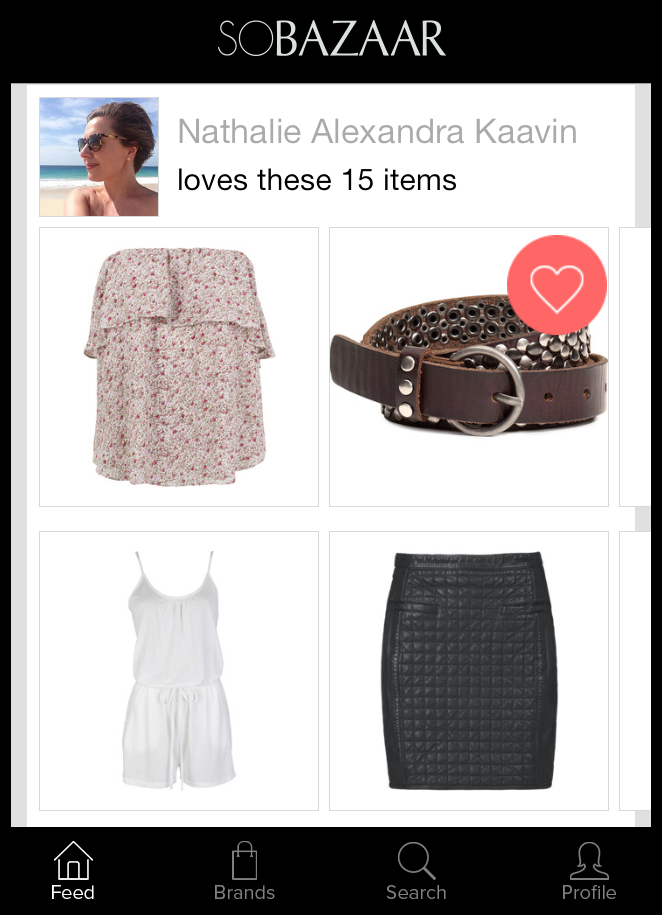
\includegraphics[height=1.5\linewidth]{image/SoBazaarfeed.png}
		\end{minipage}
		\hspace{.02\linewidth}
		\begin{minipage}{.3\linewidth}
				  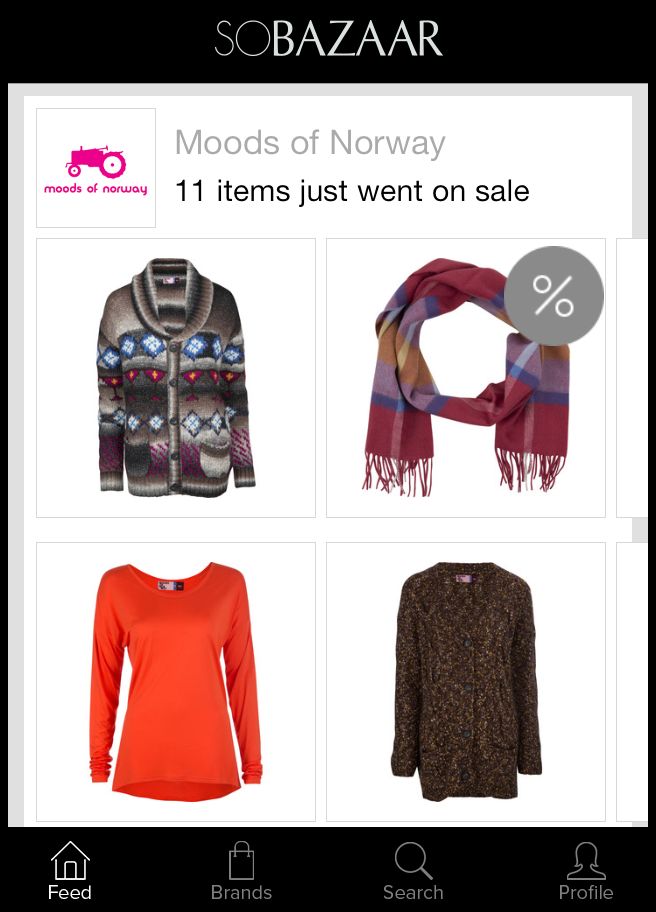
\includegraphics[height=1.5\linewidth]{image/SoBazaarsale.png}
		\end{minipage}
		\hspace{.02\linewidth}
		\begin{minipage}{.30\linewidth}
				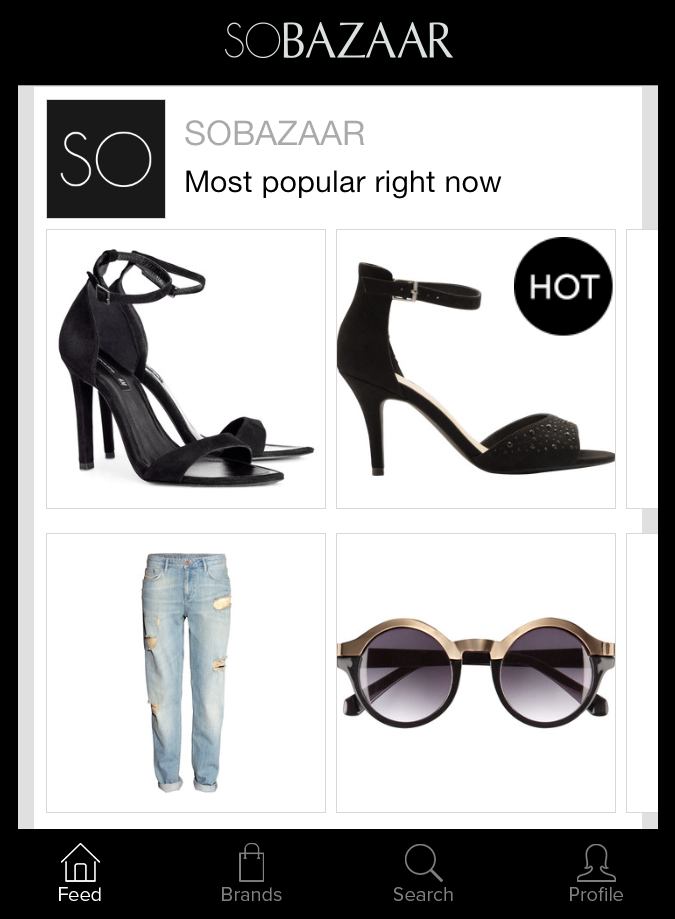
\includegraphics[height=1.5\linewidth]{image/SoBazaarmostpop.png}
		\end{minipage}
		\caption[SoBazaar newsfeed screenshots - version 0.5.1]{Screenshots from the SoBazaar Application. From the left to right: a social feed item, a sale feed item and most popular recommendations}
		\label{figure:SoBazaarfeed}
	\end{figure}

	The application brand screen shows on overview of the brands and storefront currently included in the application. The brand sceen also features an editors pick page among other things. If you find a brand you like you can choose to enter their store and view their products.

	\begin{figure}[H]
		\centering
		\begin{minipage}{.30\linewidth}
		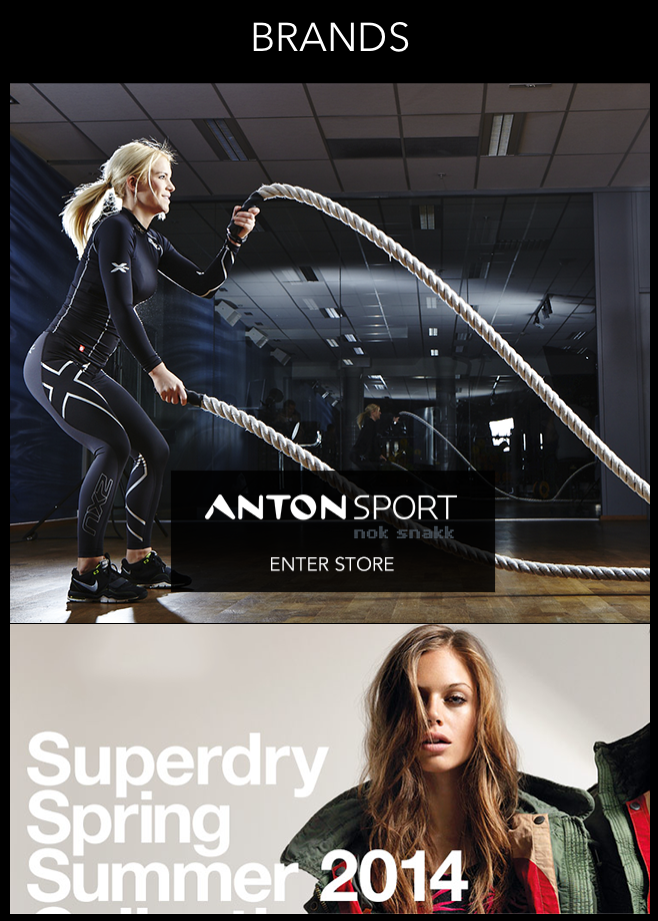
\includegraphics[height=1.5\linewidth]{image/SoBazaarbrands2.png}
		\end{minipage}
		\hspace{.02\linewidth}
		\begin{minipage}{.3\linewidth}
		  
\includegraphics[height=1.5\linewidth]{image/SoBazaareditor.png}
		\end{minipage}
		\hspace{.02\linewidth}
		\begin{minipage}{.3\linewidth}
			  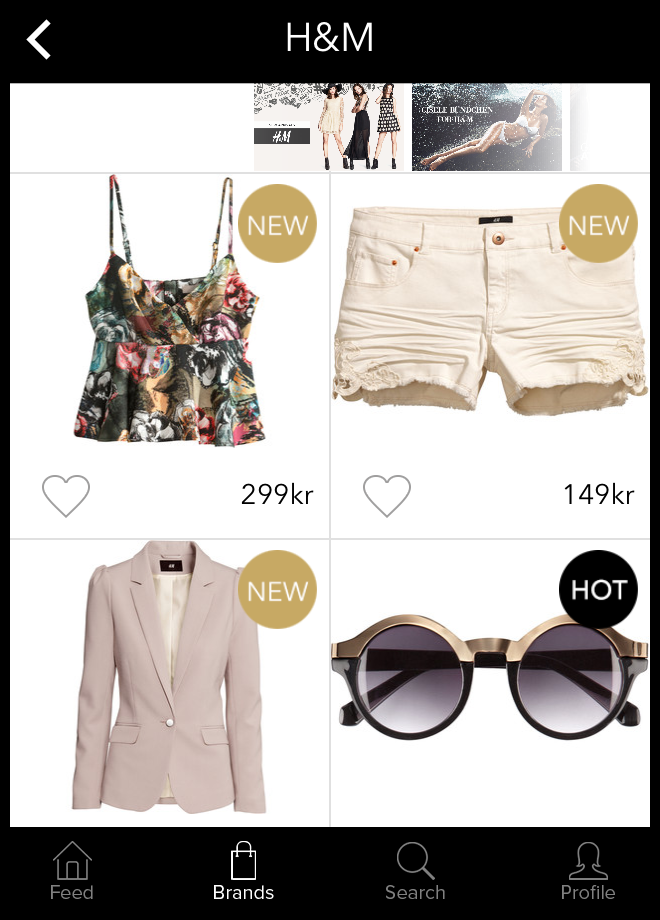
\includegraphics[height=1.5\linewidth]{image/SoBazaarStore.png}
		\end{minipage}
		\caption[SoBazaar storefront screenshots - version 0.5.1]{Screenshots from the SoBazaar Application. From the left to right: the brand browser, editors picks and the H\&M storefront}
		\label{figure:SoBazaarfeed}
	\end{figure}

	From the product screen you can choose to buy items, by being redirected to the stores online webshop. The product screen currently features a \emph{People who like this also love} widget, and also shows other products from the same store. The application also features your own personal page for your saved or \emph{loved} items. In additional the application
	also supports simple search queries.

	\begin{figure}[H]
			\centering
			\begin{minipage}{.30\linewidth}
						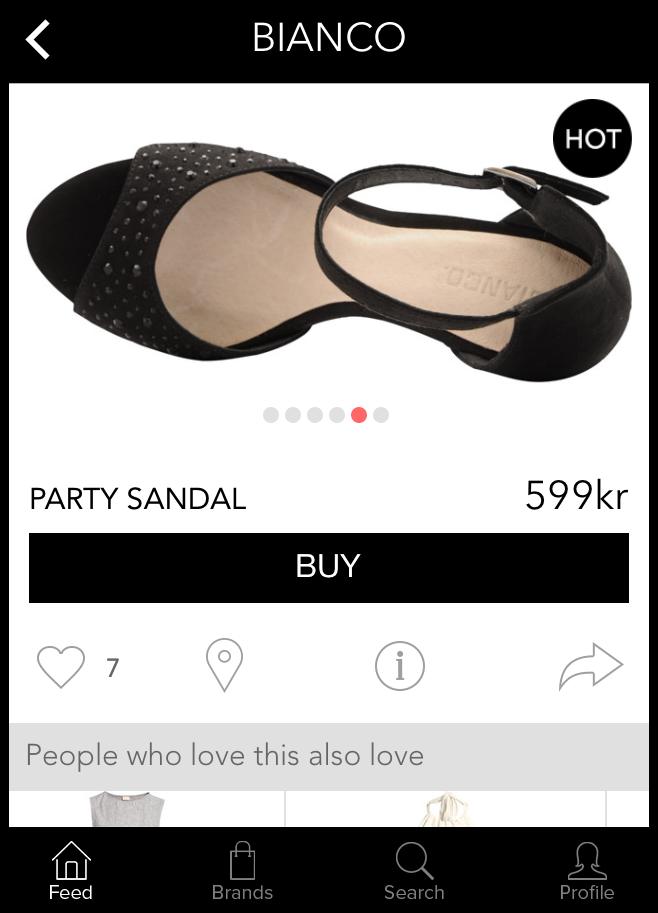
\includegraphics[height=1.5\linewidth]{image/SoBazaarproduct.png}
			\end{minipage}
			\hspace{.02\linewidth}
			\begin{minipage}{.3\linewidth}
			  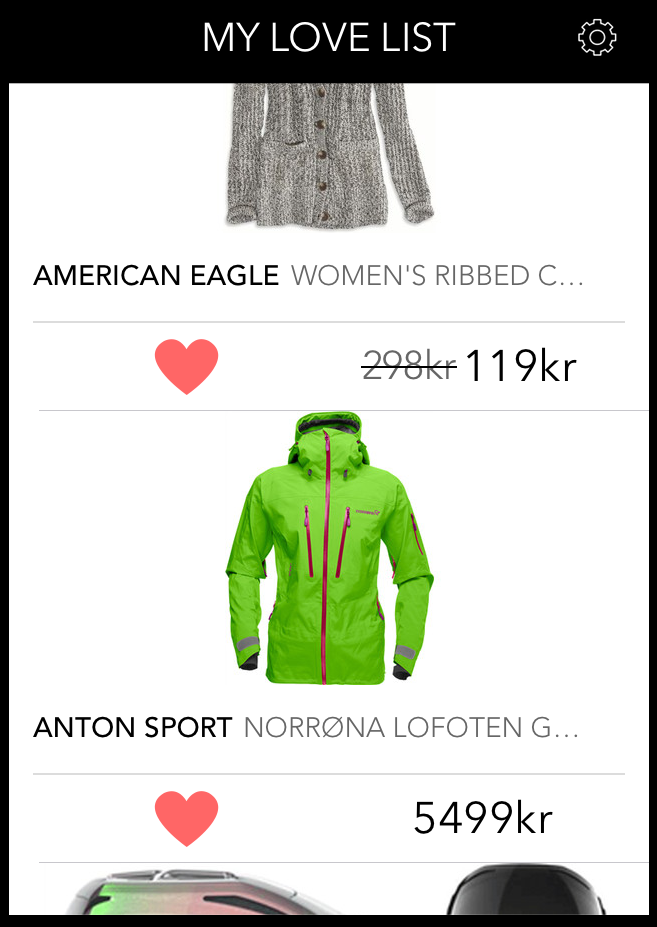
\includegraphics[height=1.5\linewidth]{image/SoBazaarlovelist.png}
			\end{minipage}
			\hspace{.02\linewidth}
			\begin{minipage}{.3\linewidth}
				  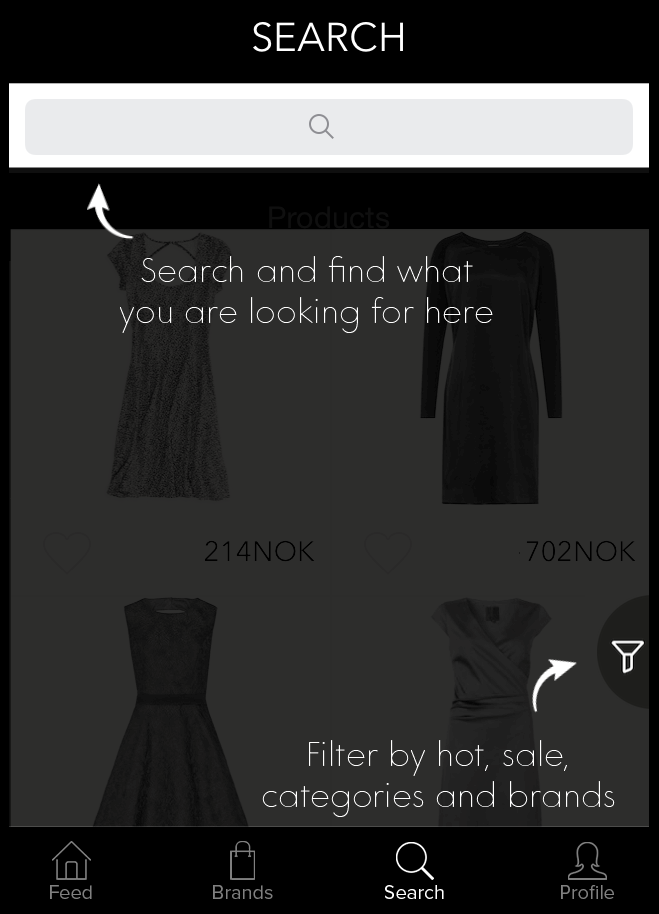
\includegraphics[height=1.5\linewidth]{image/SoBazaarsearch.png}
			\end{minipage}
			\caption[SoBazaar functionality screenshots - version 0.5.1]{Screenshots from the SoBazaar Application. From the left to right: product detail screen, the sobazar loved items list and the search screen}
			\label{figure:SoBazaarfeed}
	\end{figure}

	The application is currently in a beta phase and is planned for a final release after the summer.

\section{Preprocessing}
    \label{sec:preprocessing}
    The data from SoBazaar has been been anonymised for privacy reasons.
    In addition to anonymization the data was cleaned by removing events containing test environment flags and applications run from simulator.
    What was left after the cleaning data was mainly events triggered by the users in production environment, and not created during applications testing.

    As part of the preprocessing, an extra field was added to the data, a session field.
    This field was added to help understand how users use the application, and to be able to see use patterns.

\section{Dataset Overview}
    The data from SoBazaar is gathered based on the actions of the users using the application.
    Actions done by the users are called events, such as accessing a store, scrolling a page or purchasing a product.

    When an event is triggered a set of information is stored regarding the event.
    This data is used to make recommendations for the users though converting the implicit feedback to implicit ratings as we will see in later chapters.

    \begin{table}[H]
        \centering
        \begin{tabular}{l l}
            \toprule
            Variable     & Explanation   \\
            \midrule
            product\_id       & The id of the item which triggered the event \\
            user\_id          & The unique id of the user who triggered the event \\
            event\_id         & What kind of event was triggered~\tablefootnote{Complete list of the different types of events can be found in table~\ref{table:events}} \\
            price             & The price of the item which triggered the event \\
            retailer\_brand   & The id of the retailer brands. A retailer is a distributer of products, such as H\&M, Cubus or Moods Of Norway \\
            storefront\_id    & The storefront id of the storefront entered. The \emph{retailer\_brand}s can have multiple \emph{store\_front}s. In addition to the main \emph{store\_front} most \emph{retailer\_brands} have, they can also add one or more when there is a special occasion such as a sale or a new release \\
            event\_location   & The location of the user when the event was triggered \\
            ts                & Unix timestamp in milliseconds of when the event was triggered \\
            session           & Which session number the event belongs to~\tablefootnote{This is the value added in the preprocessing phase~\ref{sec:preprocessing}. For two events to end up in the same session, the event has to be triggered within a certain period of time, and both be after the same application started-flag} \\
            \bottomrule
        \end{tabular}
        \caption[Event Metadata]{Metadata collected from an event. The complete list can be found in table~\ref{table:completeEventData}}
        \label{table:eventData}
    \end{table}

    \begin{table}[H]
        \centering
        \begin{tabular}{l l}
            \toprule
            Attribute       & Count   \\
            \midrule
            Total number of events  &    218975 \\
            Unique users ids    &    2021 \\
            Unique item ids     &    6092 \\
            Unique storefronts  &    147~\tablefootnote{A storefront is a access point, with different clusterings of items. Stores can have multiple storefronts} \\
            Unique retailer brands  &    24 \\
            \hline
            First event & Mon, 07 Oct 2013 10:59:57 GMT \\
            Last event & Mon, 19 May 2014 22:51:19 GMT \\
            Lifetime of data & 224 days \\
            \hline
            Item clicks     &    25491 \\
            Item wants   &    13262 \\
            Item purchases   &    2020 \\
            \hline
            Average item click count per user   &    12.6130 \\
            Average item want count per user     &    6.5620 \\
            Average item purchase count per user     &    0.9995 \\
            \hline
            Average item interaction count per user     &    20.1746 \\
            Average user interaction count per item     &    6.6928 \\
            \bottomrule
        \caption[Dataset summary]{Overview of the key figures in the SoBazaar dataset}
        \label{table:datasetSummary}
        \end{tabular}
    \end{table}

    As seen from table~\ref{table:datasetSummary} the average amount of \emph{purchases} per user are below one. Using purchase information alone to make recommendations will therefore in most cases render the recommendations incomplete. If one or more users have more than one purchases, then some users will of course have none purchases. Making personalized recommendations for these users will then be unattainable.

    \emph{Clicks} and \emph{wants} on the other hand have a much higher occurrence. These two events together with \emph{purchases} tops a count of 20 on average per user, and opens for the possibility of more dense personalized recommendations, but the data is still rather sparse.

\section{Graphs}
    % Price range of items in stores
    % unique Stores count for users
    %     price span for user
    %         Timespann of sessions for users (avg, max, min)
    %         Events per session (avg, max, min)
    %         Item viewtime for user in session
    %         Stores visited per session
    %         revisit time of items for user
    %         relationship with view, want and purchase
    %         time of session over lifetime of app
    %         user preferred price in session
    %         price vs view, want and purchase
    %         avg viewtime for an item (i know)
    %         Similarity of user favorite store, items viewed and items wanted?
    %         time of session over lifetime of app for all users (slope-style)
    % user lifetimes
    This section will look at the SoBazaar data through graphing and plotting.
    It will start with the properties of the users seen in the data, then move over to the products and finally the time properties of the data.

\subsection{User properties}
    \begin{figure}[H]
        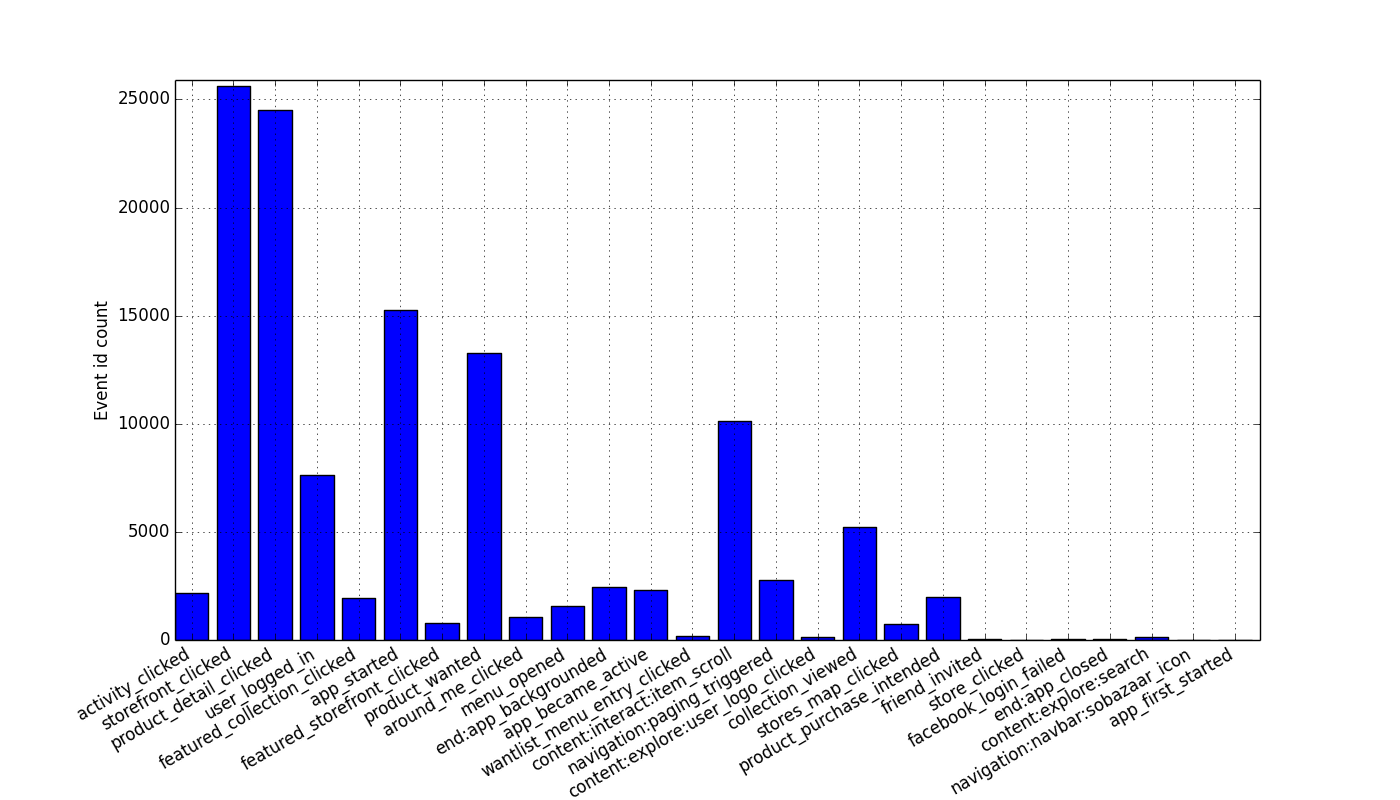
\includegraphics[width=5in]{image/event_iddistribution.png}
        \centering
        \caption{Count for different events}
    \label{figure:eventIDDistribution}
    \end{figure}
        In the figure above (figure~\ref{figure:eventIDDistribution}) we see the count for each of the different events which can be triggered in the SoBazaar application.
        As seen from the graph the \emph{product\_detail\_clicked}-event and the \emph{storefront\_clicked}-event are the two most common events to be triggered.
        As mentioned earlier in~\ref{table:eventData}, the \emph{storefront} is the main access point to a set of products, and the high values for this \emph{event\_id} is as expected.
        The fact that accessing the \emph{storefront} is the most occurring event, over clicking an item, indicates that many users browse the items through looking at the thumbnails rather than accessing the actual item.

        The \emph{product\_wanted}-event is the fourth most occurring event, and is about half the size of the \emph{product\_detail\_clicked}-event, this does not mean that half of the accessed items are added to a want list, since it is possible to want an item without accessing the item.
        \emph{product\_purchase\_intended} on the other hand has to come after a \emph{product\_detail\_clicked}, so it is therefore safe to assume that about 8\% of item accesses progressed into an intended purchase.

    \begin{figure}[H]
        \centering
        \begin{subfigure}{.5\textwidth}
            \centering
            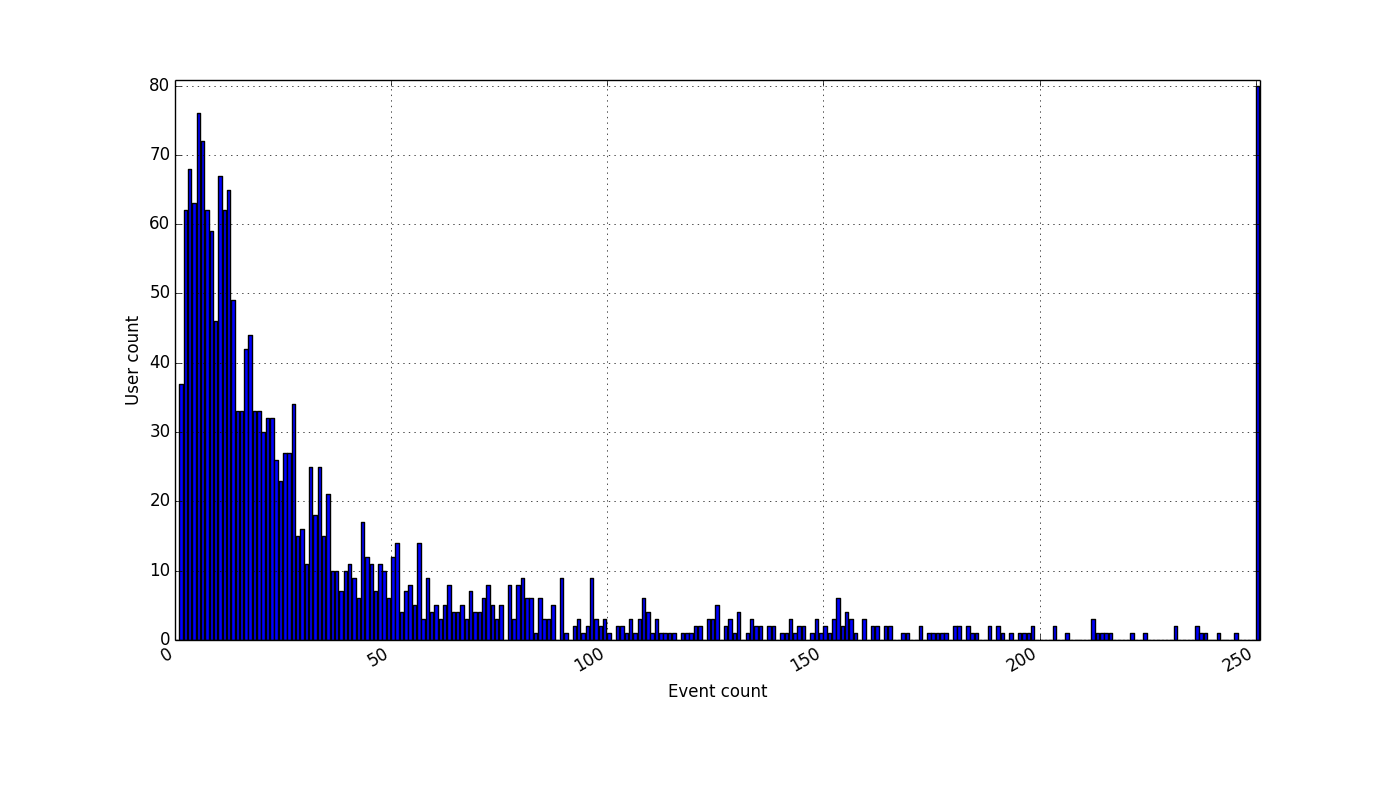
\includegraphics[width=\dualGraphWidth]{image/user_iddistribution.png}
            \caption{Distribution of events on users}
    \label{figure:userEventDist}
        \end{subfigure}%
        \begin{subfigure}{.5\textwidth}
            \centering
            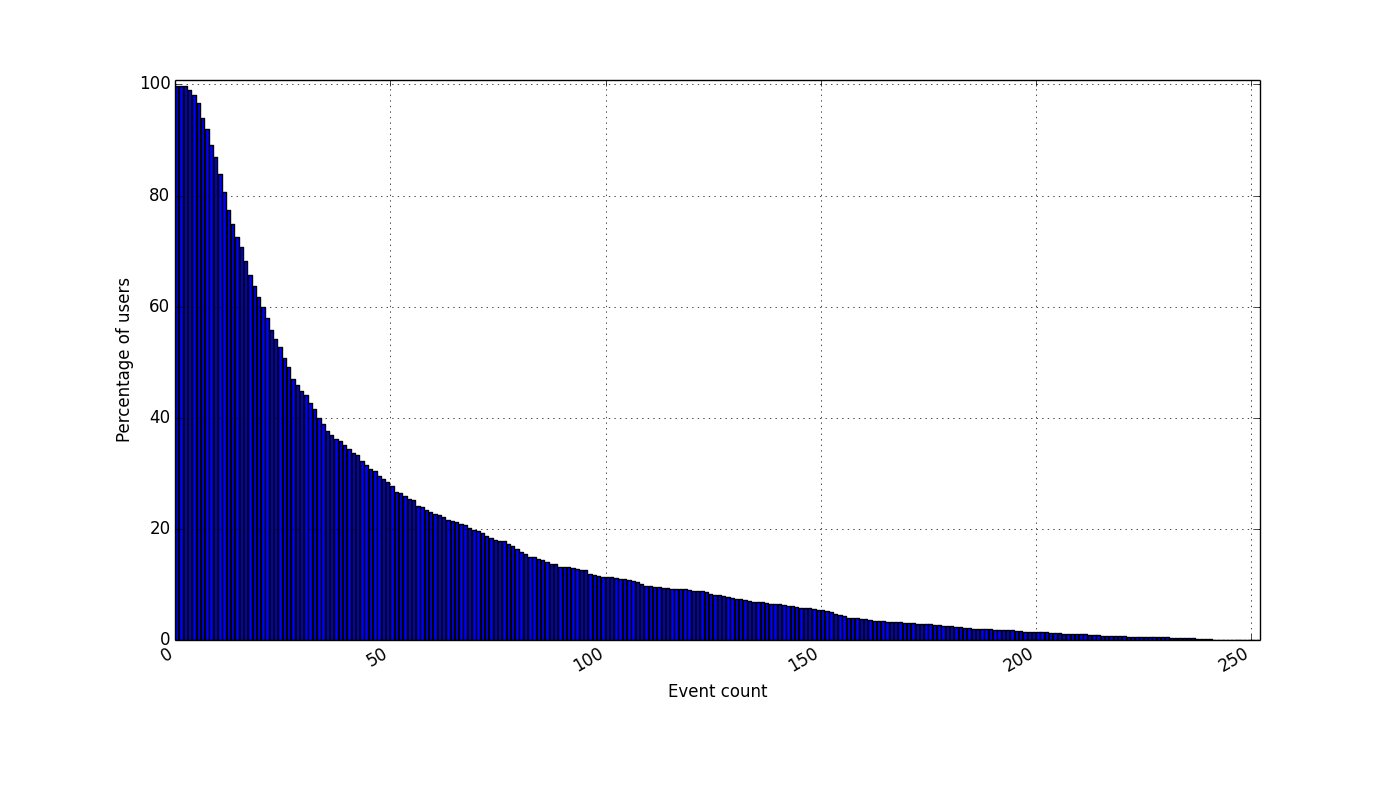
\includegraphics[width=\dualGraphWidth]{image/user_idcumdistribution.png}
            \caption{Cumulative distribution of events on users}
    \label{figure:userEventCumDist}
        \end{subfigure}
        \caption{Graphs presenting the distribution of events per user}
    \end{figure}
        Figure~\ref{figure:userEventDist} is showing the actual amount of users with the different counts of events.
        78\% of the users have 50 or less events, with the most common amount being at 5 events.
        The figures are showing the values from 0 to 250 since 96\% of the users reside in this subset.
        Max count of events for one user is 6055.

        As seen from figure~\ref{figure:eventIDDistribution} most of the events are not directly related to products, from table~\ref{table:datasetSummary} we can see that there are over 6000 products, and as mentioned above, 78\% of the users have less than 50 events. Based on these three facts, we can assume that the data is sparse.

    \begin{figure}[H]
        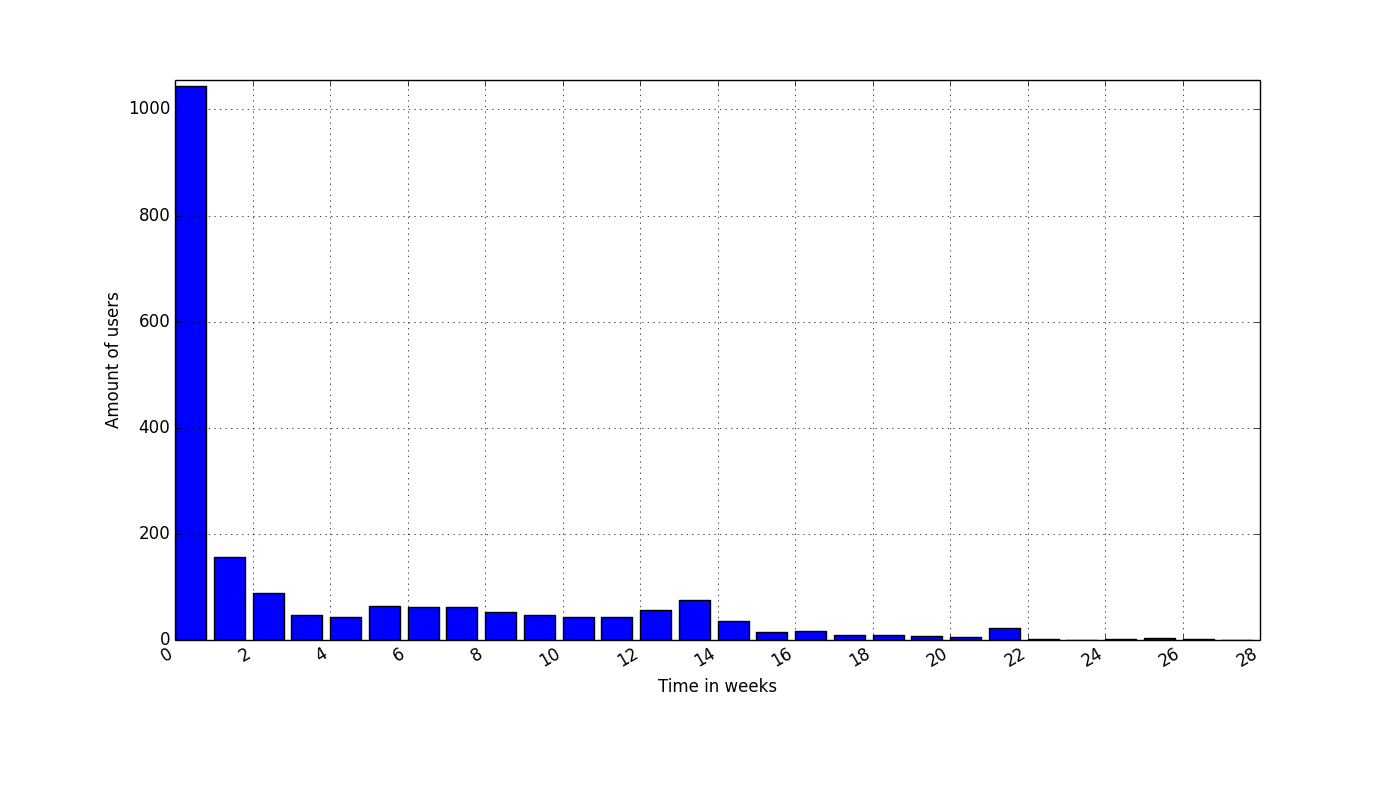
\includegraphics[width=5in]{image/userTimespansdistribution.png}
        \centering
        \caption{Distribution of user account lifetime}
    \label{figure:userTimespandist}
    \end{figure}

    %mtodo

    \begin{figure}[H]
        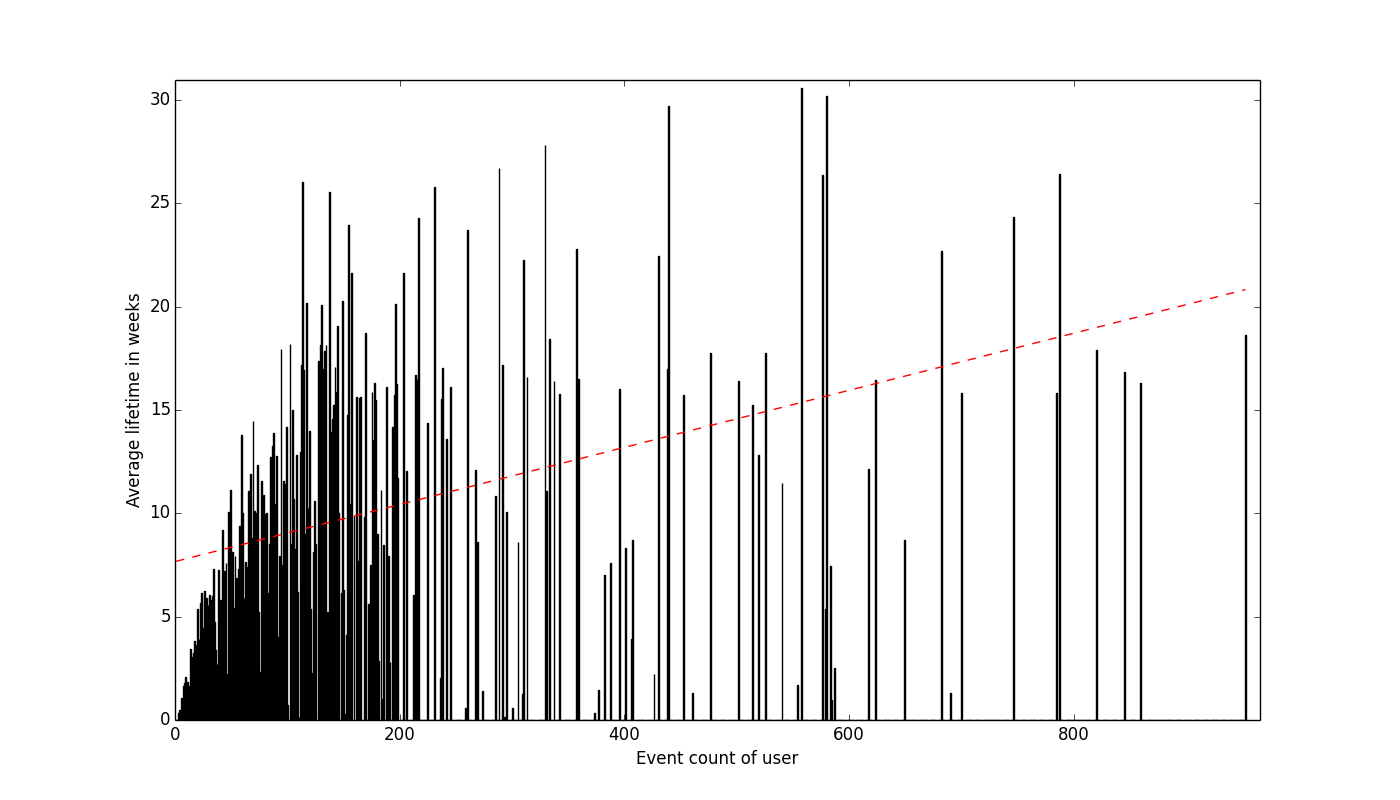
\includegraphics[width=5in]{image/avglifetimeoncountuser.png}
        \centering
        \caption{Average lifetime of user accounts sorted on event count}
    \label{figure:avglifetimeoncountuser}
    \end{figure}

    %mtodo

    \begin{figure}[H]
        \centering
        \begin{subfigure}{.5\textwidth}
            \centering
            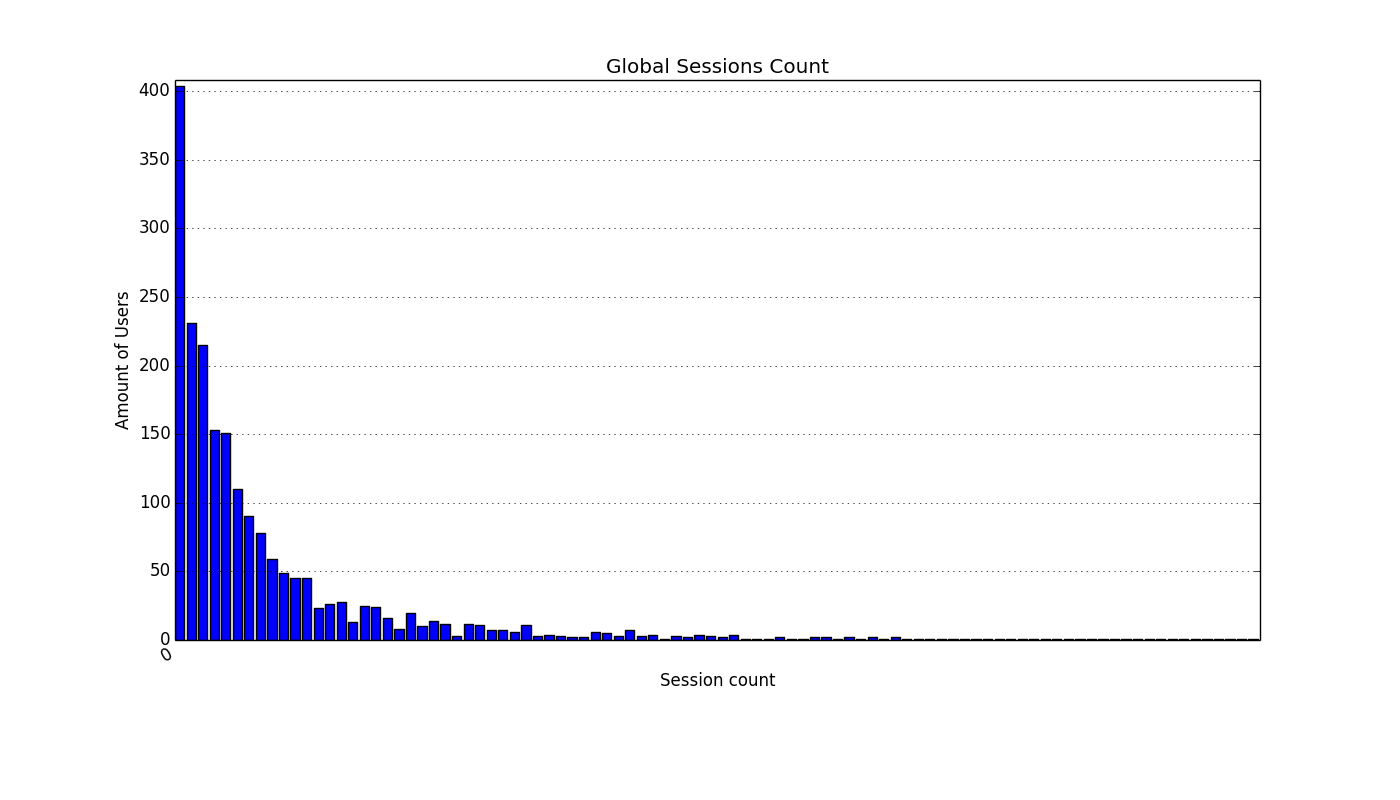
\includegraphics[width=\dualGraphWidth]{image/sessionsCountdistribution.png}
            \caption{Distribution of sessions for users}
    \label{figure:sessCountDist}
        \end{subfigure}%
        \begin{subfigure}{.5\textwidth}
            \centering
            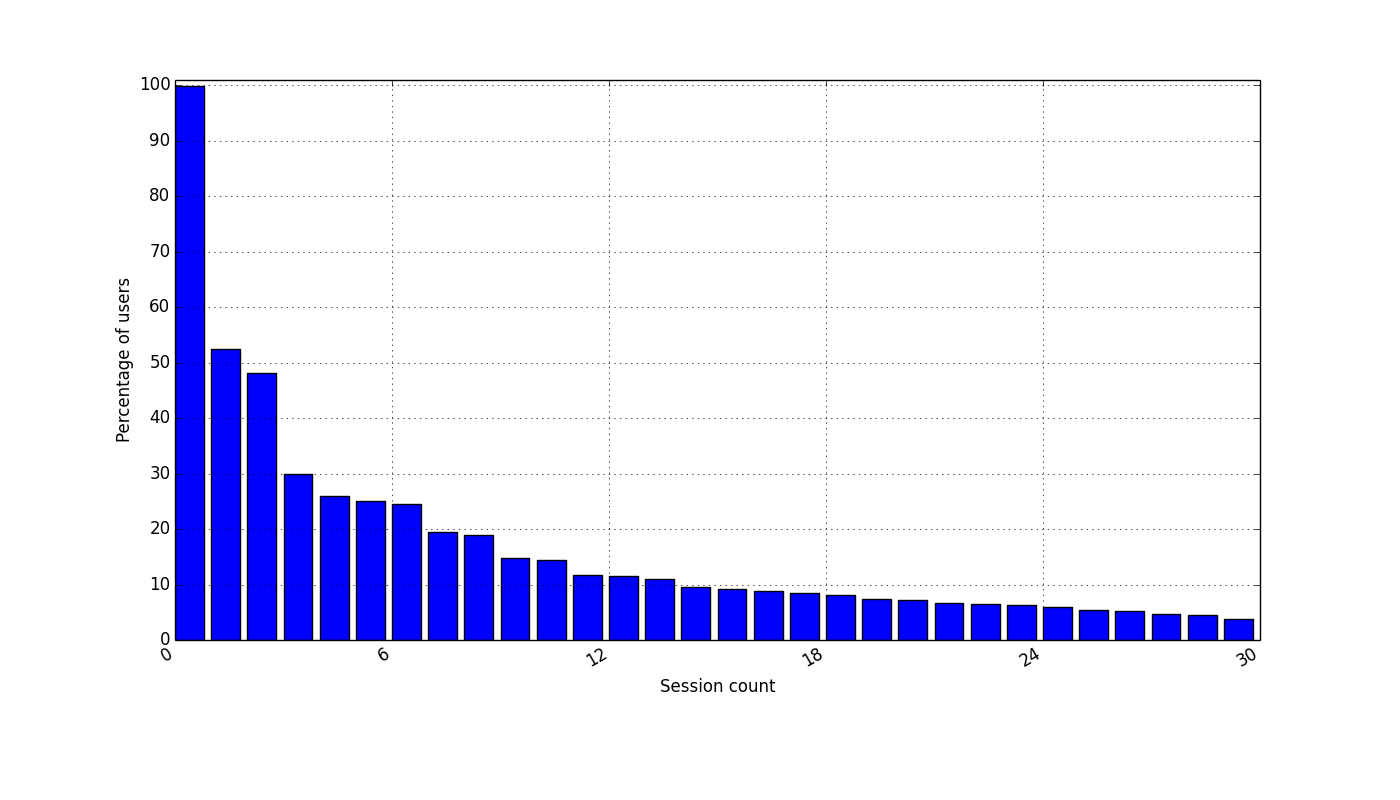
\includegraphics[width=\dualGraphWidth]{image/sessioncumdistribution.png}
            \caption{Cumulative distribution of sessions for users}
    \label{figure:sessCountCumDist}
        \end{subfigure}
        \caption{Graphs presenting the number of sessions for the users in the data}
    \end{figure}
        \marginpar{Something wrong with sessions graphs, will fix}
        % mtodo
        More than 90\% of the users of SoBazaar have a session count of 20 and less.
        This means that they have not used the applications more than 20 separate times, over the time the data was collected, and strengthens the hypothesis that the data from SoBazaar is sparse.

        The maximum number of sessions for each user is grouped to show the count of how many users has the different amount of sessions.

        In figure~\ref{figure:sessCountDist} the 4 first bars sums up to 1000, which is the amount of users who has had 4 or less sessions on the application in total. In other words --- half of the user base used the application less than 4 times.


    \begin{figure}[H]
        \centering
        \begin{subfigure}{.5\textwidth}
            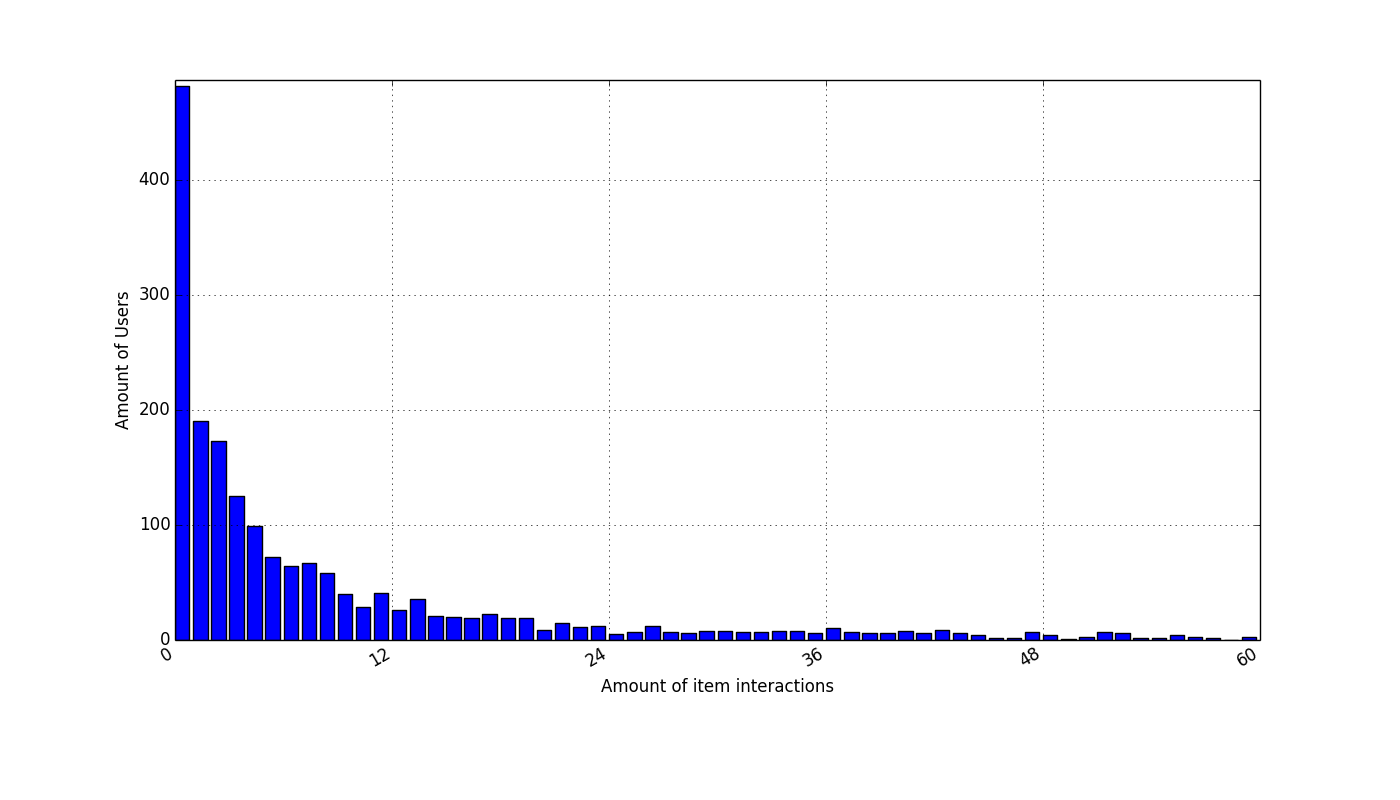
\includegraphics[width=\dualGraphWidth]{image/ratingsPerUserdistribution.png}
            \centering
            \caption{Count of item interactions for users}
    \label{figure:ratingsPerUser}
        \end{subfigure}%
        \begin{subfigure}{.5\textwidth}
            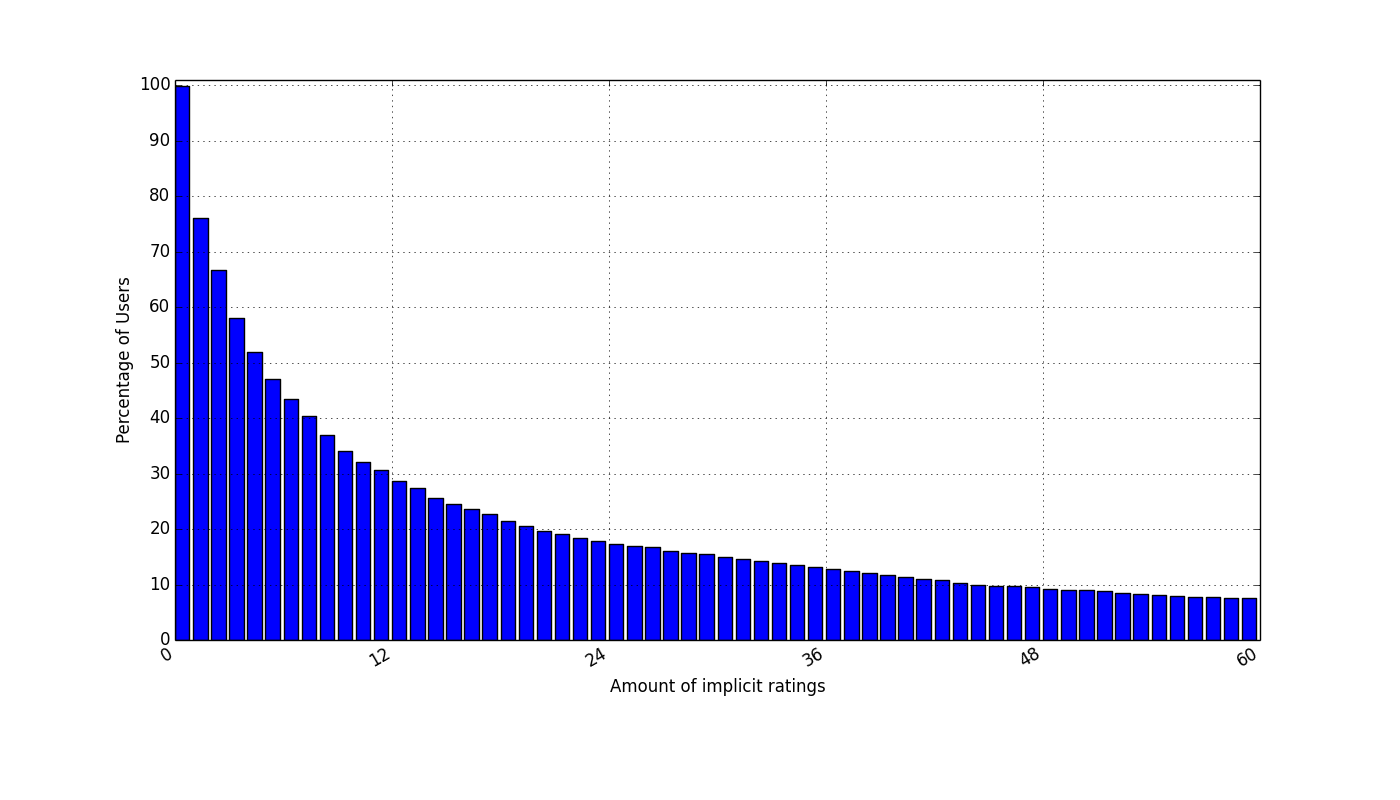
\includegraphics[width=\dualGraphWidth]{image/ratingsPerUsercumdistribution.png}
            \centering
            \caption{Cumulative count of item interactions for users}
    \label{figure:ratingsPerUserCum}
        \end{subfigure}
        \caption{Figures presenting the number of product interactions for the users in the data}
    \end{figure}
        In the figures above the rightmost bar present 0 product interactions.
        The graphs are limited to only showing interaction amounts up till 60 to give focus to the numbers where more than 90\% of the users resides.

        As seen from figure~\ref{figure:ratingsPerUserCum}, over 20\% of the users have never interacted with an item, and about 10\% of the users have more than 50 item interactions.

        Even though the data is sparse, as seen from the previous figures, the fact that the majority of the users have in some way interacted with items, opens for the possibility of drawing conclusions based on other users' item interactions.

    \begin{figure}[H]
        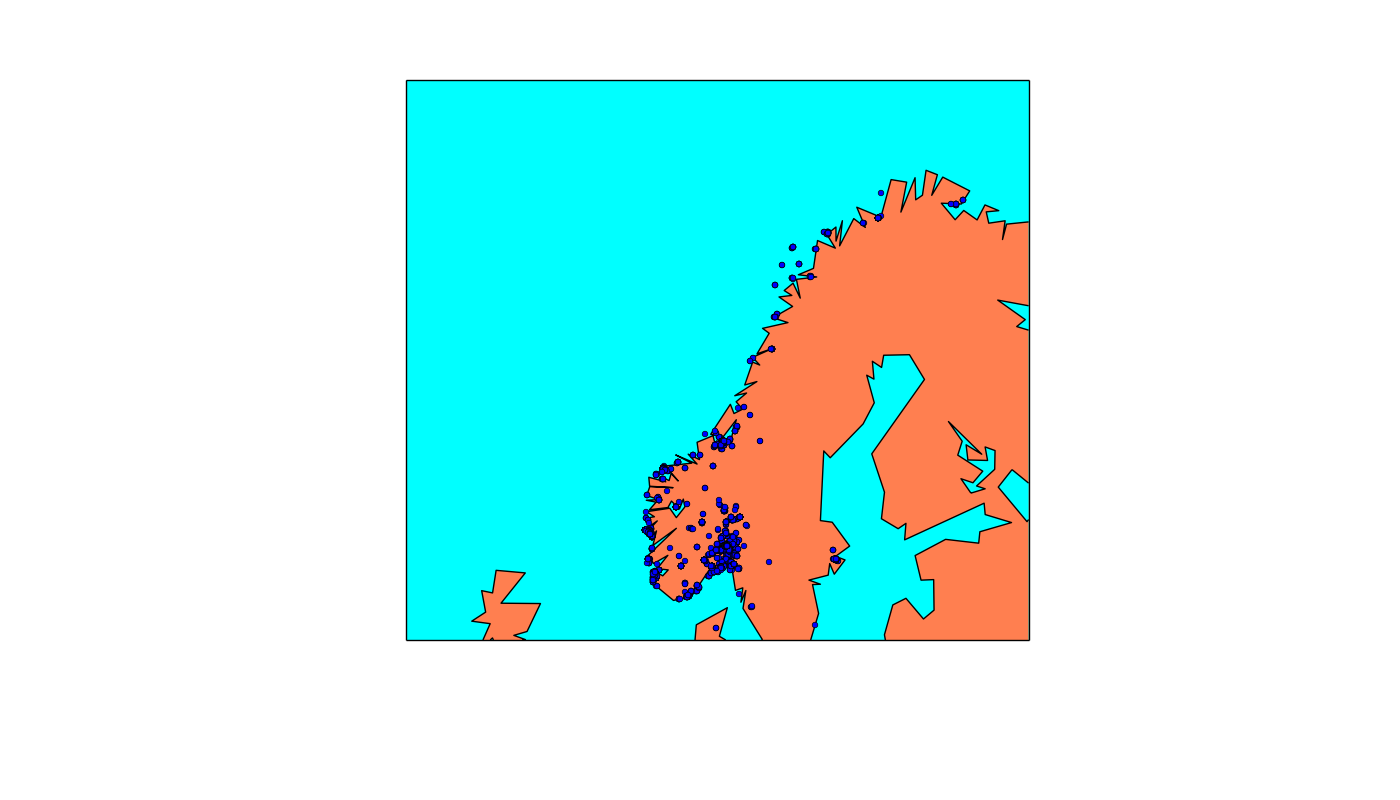
\includegraphics[width=5in]{image/simpleGeoPlotNorway.png}
        \centering
        \caption{Plot of event location in and around Norway}
    \label{figure:croppedGeoplot}
    \end{figure}
        Figure~\ref{figure:croppedGeoplot} shows the location of the user at the time the different events was triggered.
        It is cropped to show events triggered in and around Norway.
        We can see that the majority of the users are located in and around the capital city of Norway, Oslo.

        If the event is triggered from a phone, the event is as precise as the GPS hardware location of the phone, and would be helpful information to understand more about the user.

        % mtodo check for price distribution based on location.

\subsection{Product properties}

    \begin{figure}[H]
        \centering
        \begin{subfigure}{.5\textwidth}
            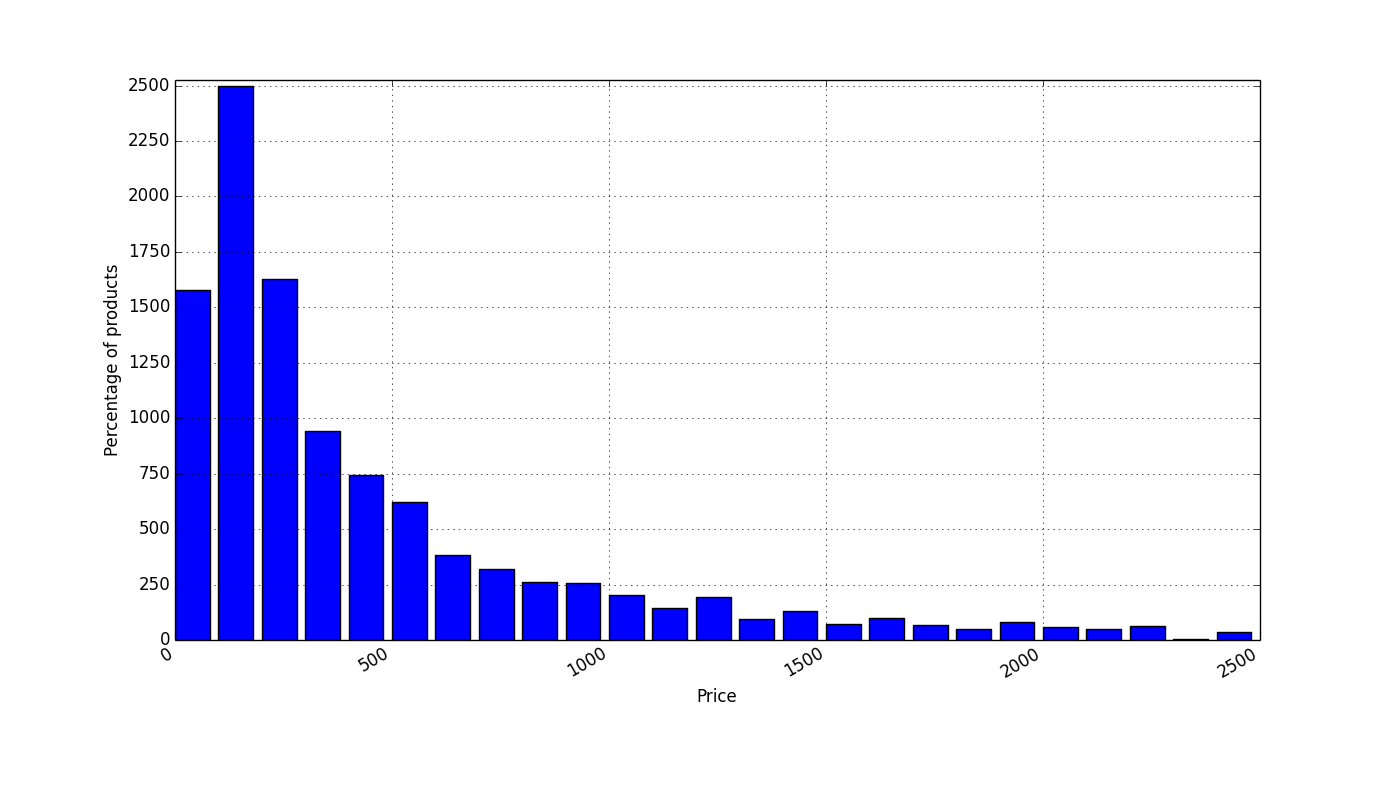
\includegraphics[width=\dualGraphWidth]{image/priceDistributiondistribution.png}
            \centering
            \caption{Price distribution of products}
    \label{figure:pricePerProduct}
        \end{subfigure}%
        \begin{subfigure}{.5\textwidth}
            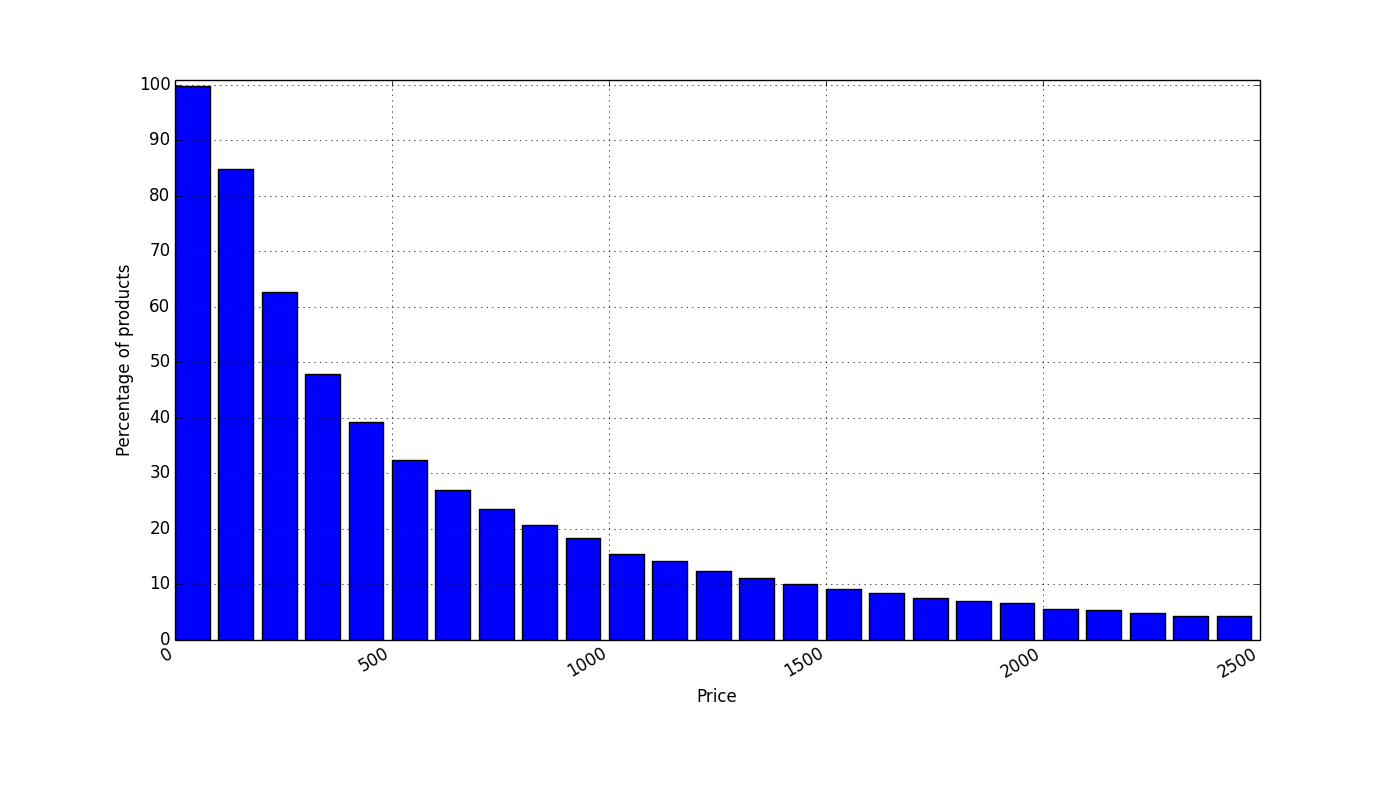
\includegraphics[width=\dualGraphWidth]{image/cumpriceDistributiondistribution.png}
            \centering
            \caption{Cumulative price distribution of products}
    \label{figure:pricePerProductCum}
        \end{subfigure}
        \caption{Figures presenting the distribution of price for the items i SoBazaar}
    \end{figure}

        Here we see how the products are distributed in regards to their price.
        134 products have a price over 2 500 NOK and have been left out of this graph.

        82\% of the items have a price lower than 1 000 NOK.
        \marginpar{make avg price for users, is there something there}
        % mtodo make price user graph

    \begin{figure}[H]
        \centering
        \begin{subfigure}{.5\textwidth}
            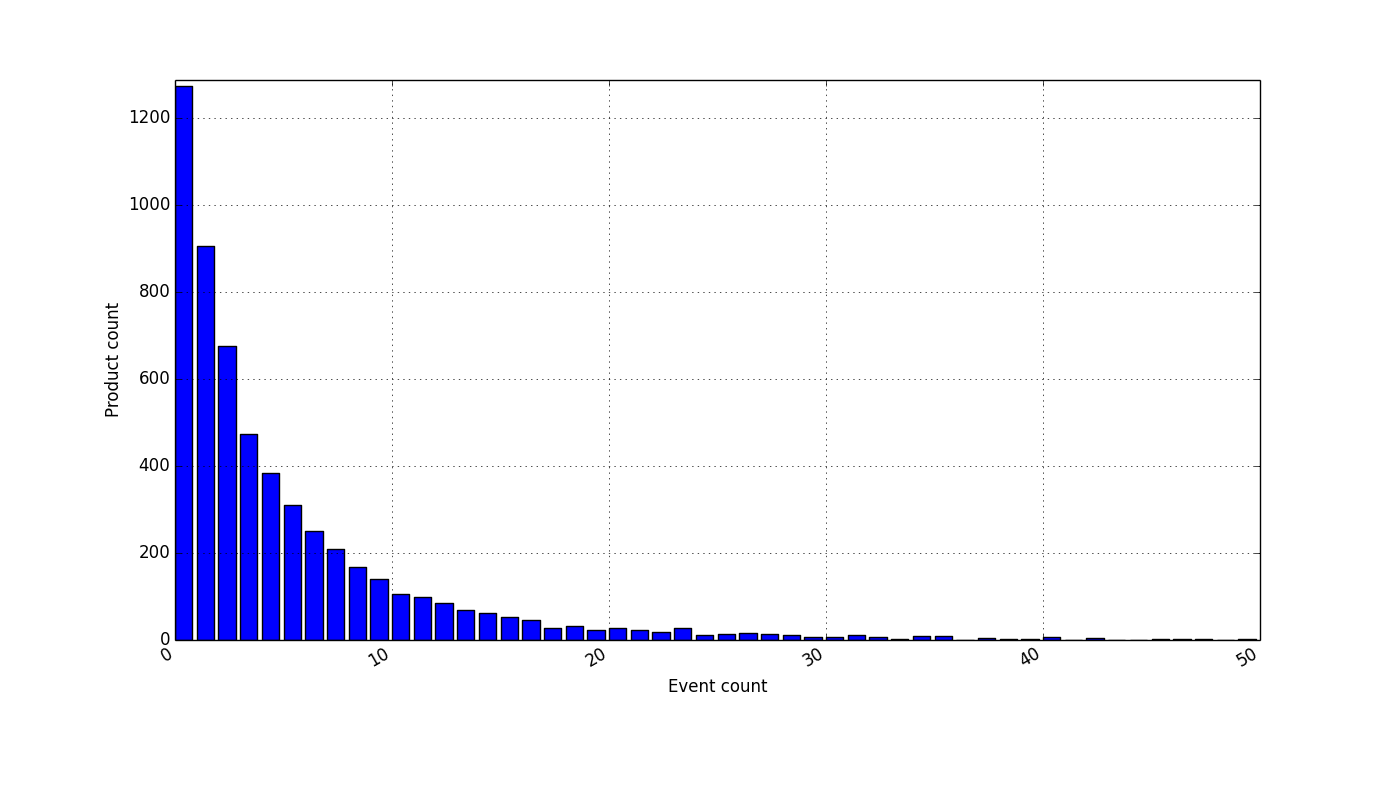
\includegraphics[width=\dualGraphWidth]{image/product_iddistribution.png}
            \centering
            \caption{Count of events on products}
    \label{figure:eventsPerproduct}
        \end{subfigure}%
        \begin{subfigure}{.5\textwidth}
            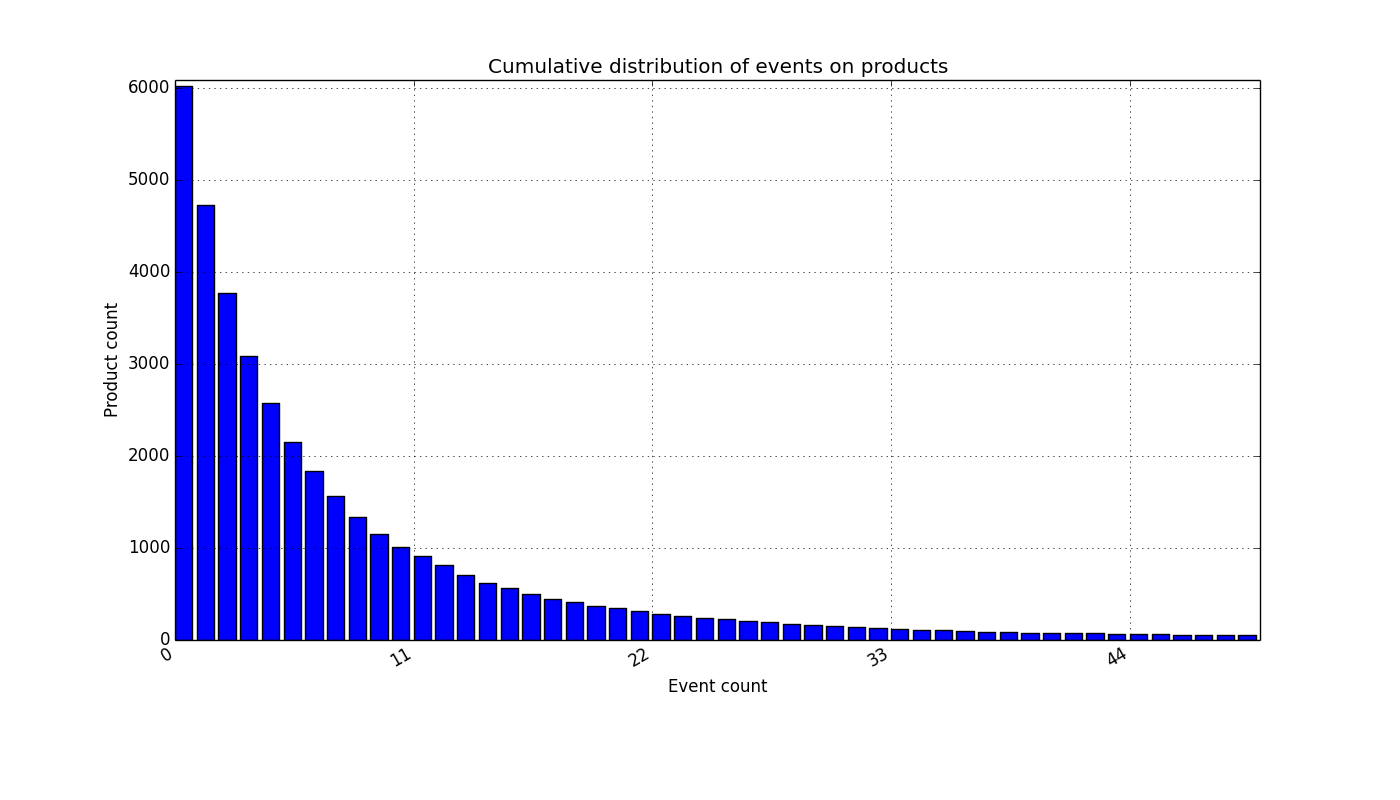
\includegraphics[width=\dualGraphWidth]{image/product_idcumdistribution.png}
            \centering
            \caption{Cumulative count of events on products}
    \label{figure:eventsPerproductCum}
        \end{subfigure}
        \caption{Figures presenting the distribution of events for the products i SoBazaar}
    \end{figure}
        80\% of the products have only a interaction count of 10 or less.
        Interaction count is \emph{product\_detail\_clicked}, \emph{product\_wanted} and \emph{product\_purchase\_intended}.
        This means that there will not be more than 10 events for the majority of the items, which leads to an issue when doing collaborative filtering on the data.
        When the majority of the events only has 10 events and there are over 4 000 items and 1 200 users, the probability that multiple users have interacted with similar items will be marginal.

\subsubsection{The Pareto principle and Long tail on sales}
    In e-commerce the distribution of sales or product interactions can be described by the Pareto principle and the phenomenon of long tail.
    Pareto's principle is used to tell how the distribution is in the \emph{head}~\footnote{Take for example figure~\ref{figure:eventsPerproduct}, the \emph{head} is the left most part where the curve is steep} of the graph, and the long tail phenomenon is used to tell tell how the distribution is in the \emph{tail}~\footnote{Take for example figure~\ref{figure:eventsPerproduct}, the \emph{tail} is the right most part where the curve flattens out} of the graph.

    \marginpar{maybe add a figure showing head and tail of a graph instead of a footnote explaining}

\paragraph{Pareto's Principle}
    Pareto's principle applies when the 20\% most frequent products account for more than 80\% of the ratings, sales or interactions in the dataset~\cite{newman05power}.

    \begin{figure}[H]
        \centering
        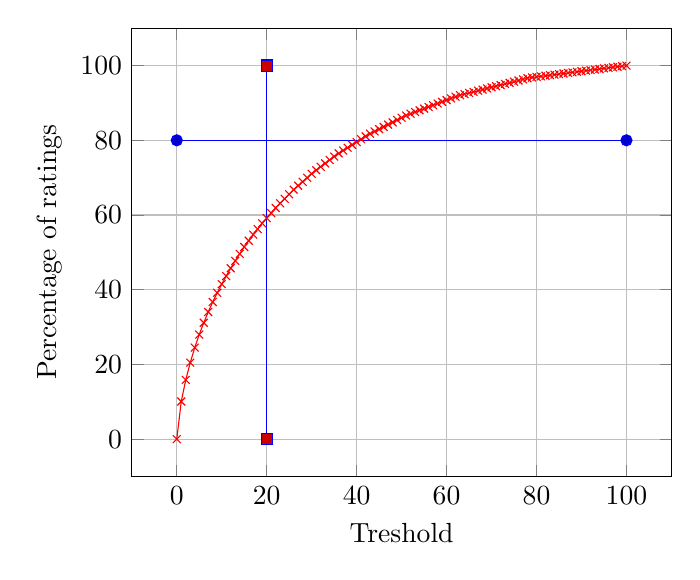
\begin{tikzpicture}
            \begin{axis}[
                xlabel=Treshold,
                ylabel=Percentage of ratings,
                grid=major,
            ]
            \addplot+[color=blue,sharp plot] coordinates
                {(0,80) (100,80)};
            \addplot+[color=blue,sharp plot] coordinates
                {(20,0) (20,100)};
            \addplot[color=red,mark=x] coordinates {
                    (0.0, 0.0)
                    (1.0, 10.089827139370456)
                    (2.0, 15.879525954256096)
                    (3.0, 20.48914274211811)
                    (4.0, 24.52004126512845)
                    (5.0, 28.004931686083083)
                    (6.0, 31.16775281181592)
                    (7.0, 34.053795636967514)
                    (8.0, 36.72848048712981)
                    (9.0, 39.184258863196035)
                    (10.0, 41.49409958986488)
                    (11.0, 43.66303499987419)
                    (12.0, 45.76151775155373)
                    (13.0, 47.72412751931158)
                    (14.0, 49.60370379689505)
                    (15.0, 51.44553757894472)
                    (16.0, 53.116272047907806)
                    (17.0, 54.75178018770601)
                    (18.0, 56.2614800090582)
                    (19.0, 57.79634149409959)
                    (20.0, 59.17016833153008)
                    (21.0, 60.52889817074705)
                    (22.0, 61.887628009964025)
                    (23.0, 63.14571119442417)
                    (24.0, 64.35347105150593)
                    (25.0, 65.56123090858767)
                    (26.0, 66.78912009662079)
                    (27.0, 67.84842613793623)
                    (28.0, 68.90521601288278)
                    (29.0, 69.9620058878293)
                    (30.0, 71.03640892735828)
                    (31.0, 72.00261681302368)
                    (32.0, 72.90843670583499)
                    (33.0, 73.8142565986463)
                    (34.0, 74.73517348967114)
                    (35.0, 75.64099338248245)
                    (36.0, 76.49900611428427)
                    (37.0, 77.25385602496037)
                    (38.0, 78.02128676748107)
                    (39.0, 78.77613667815716)
                    (40.0, 79.53098658883326)
                    (41.0, 80.29841733135395)
                    (42.0, 81.05326724203005)
                    (43.0, 81.77540698991017)
                    (44.0, 82.37928691845104)
                    (45.0, 82.9932315124676)
                    (46.0, 83.59711144100848)
                    (47.0, 84.20099136954934)
                    (48.0, 84.80487129809023)
                    (49.0, 85.41881589210678)
                    (50.0, 86.02269582064767)
                    (51.0, 86.62657574918853)
                    (52.0, 87.11974435749693)
                    (53.0, 87.57265430390258)
                    (54.0, 88.02556425030824)
                    (55.0, 88.47847419671389)
                    (56.0, 88.9389326422263)
                    (57.0, 89.39184258863196)
                    (58.0, 89.84475253503761)
                    (59.0, 90.29766248144327)
                    (60.0, 90.75812092695568)
                    (61.0, 91.21103087336134)
                    (62.0, 91.66394081976699)
                    (63.0, 92.06149510605641)
                    (64.0, 92.36343507032684)
                    (65.0, 92.66537503459729)
                    (66.0, 92.96731499886772)
                    (67.0, 93.27428729587601)
                    (68.0, 93.57622726014644)
                    (69.0, 93.87816722441687)
                    (70.0, 94.18010718868732)
                    (71.0, 94.48707948569559)
                    (72.0, 94.78901944996603)
                    (73.0, 95.09095941423647)
                    (74.0, 95.39289937850691)
                    (75.0, 95.69987167551518)
                    (76.0, 96.00181163978563)
                    (77.0, 96.30375160405606)
                    (78.0, 96.61072390106435)
                    (79.0, 96.8170495433158)
                    (80.0, 96.96801952545103)
                    (81.0, 97.11898950758624)
                    (82.0, 97.27247565609038)
                    (83.0, 97.4234456382256)
                    (84.0, 97.57441562036082)
                    (85.0, 97.72538560249603)
                    (86.0, 97.87887175100018)
                    (87.0, 98.0298417331354)
                    (88.0, 98.18081171527061)
                    (89.0, 98.33429786377475)
                    (90.0, 98.48526784590997)
                    (91.0, 98.6362378280452)
                    (92.0, 98.7872078101804)
                    (93.0, 98.94069395868455)
                    (94.0, 99.09166394081976)
                    (95.0, 99.24263392295498)
                    (96.0, 99.3936039050902)
                    (97.0, 99.54709005359435)
                    (98.0, 99.69806003572957)
                    (99.0, 99.84903001786478)
                    (100.0, 100.0)
            };
            \end{axis}
        \end{tikzpicture}
        \caption{Pareto's principle values graphed}
    \label{figure:paretosPrinciple}
    \end{figure}

    \begin{table}[H]
        \centering
        \begin{tabular}{lll}
        \toprule
        Threshold &   Products in threshold~\tablefootnote{The amount of products residing within the percentage threshold} &      Percentage of interactions \\
        \midrule
        20\%    &    1206   &    59.1701\% \\
        41\%    &    2472   &    80.2984\% \\
        \bottomrule
        \end{tabular}
        \caption{Pareto's principle values}
    \label{table:paretosPrinciple}
    \end{table}

    Figure~\ref{figure:paretosPrinciple} show the percentages of interactions within the given thresholds.
    As we can see from table~\ref{table:paretosPrinciple}, the 20\% most frequently interacted with items represents 59.1701\% of the ratings.
    We have to move up to 41\% to reach 80\% of the interactions, and the Pareto's principle does therefore not apply to the SoBazaar.

\paragraph{Long Tail}
    The definition of long tail is that the most frequently-occuring items represent less than 50\% of occurrences in logs~\cite{DBLP:journals/corr/abs-1203-4487}.

    \begin{table}[H]
        \centering
        \begin{tabular}{llll}
        \toprule
        Average product interaction   & Products in threshold~\tablefootnote{The amount of product residing within the percentage threshold} & Coverage & Percentage of interactions \\
        \midrule
        6.6928   &    4194   & 68.8443\% &   28.5408\% \\
        \bottomrule
        \end{tabular}
        \caption{Long tail values}
    \label{table:longtail}
    \end{table}

    As the table above shows the SoBazaar data does not posses a clear long tail behavior.
    The average interaction count of the products is 6.6928 and there is 4194 products with less than this number of interactions, but these items does only cover 28.5408\% of the total interactions.

    % mtodo - price for store dist
    \begin{figure}[H]
        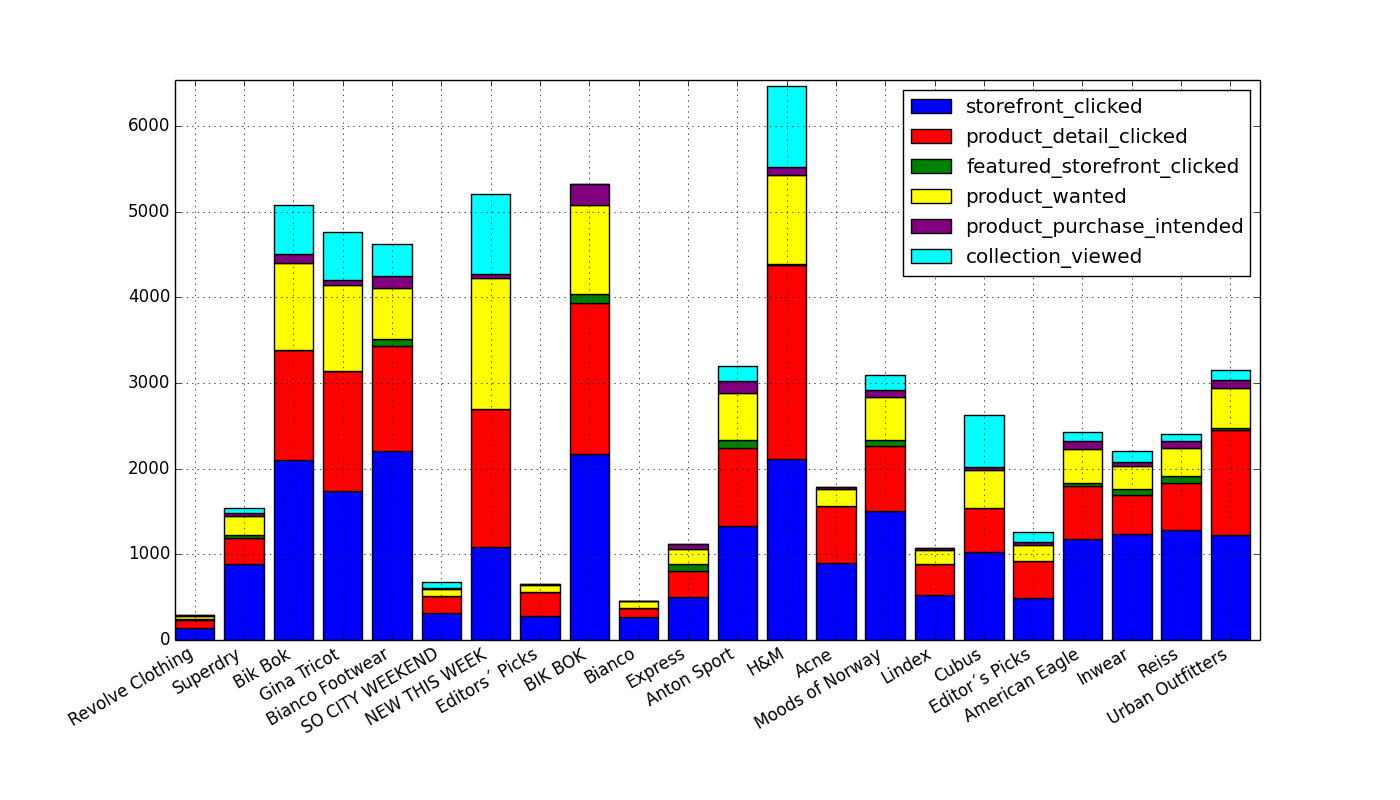
\includegraphics[width=5in]{image/storefront_nameandEventdistribution.png}
        \centering
        \caption{Distribution of events on storefronts}
    \label{figure:eventOnStoreFrontDist}
    \end{figure}
        \marginpar{sort it}
        The events triggered in context with the different storefronts.
        The events are segmented to show the different event counts on the different storefronts, and stacked to show the complete count, to be able to clearly see how the events are distributed over the different stores.
        We can see that \emph{H\&M} is the most popular store in total, but \emph{BIK BOK} has the most \emph{product\_purchase\_intended}-events.
        One interesting find to take from this graph is the \emph{storefront\_clicked} to the item interaction related events (\emph{product\_detail\_clicked}, \emph{product\_wanted} and \emph{product\_purchase\_intended}) ratio.
        For instance \emph{Bik Bok} has a much higher item interaction count than storefront access count, whereas stores such as \emph{Reiss} and \emph{Inwear} are mostly accessed and the items not interacted with.
        Different aspects affecting this might be price, style and item presentation.

\subsection{Time properties}

    % mtodo - si noe om hvorfor ikke? jeg vil vel påstå at dette sier no om viktihet av "nyhetsverdi" for item'et, og ville derfor trodd dette var relevant info?
    % mtodo - fix while watching AT wooo
    % Why is this important, clearify text, what can we learn from the plots?
    \begin{figure}[H]
        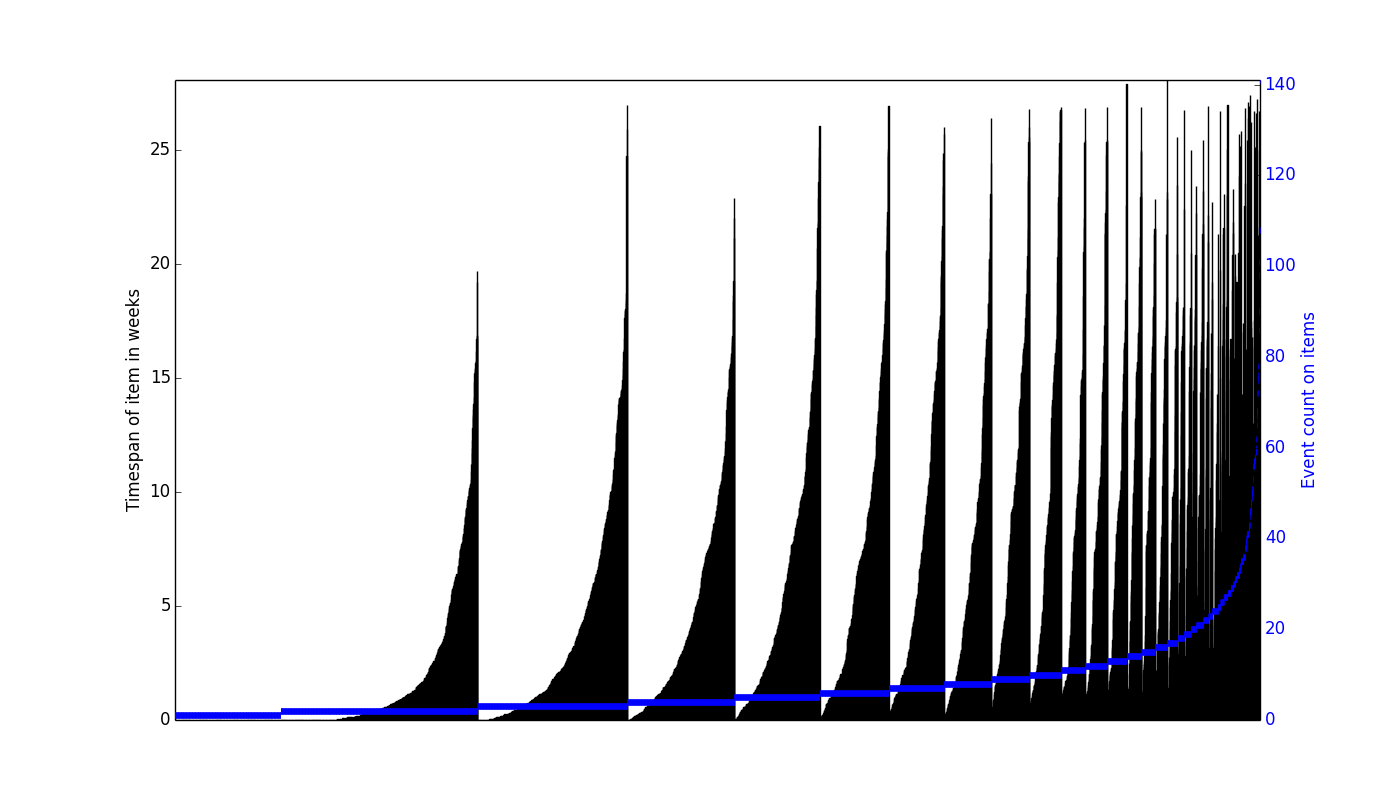
\includegraphics[width=5in]{image/itemTimeSpansortedoneventcount.png}
        \centering
        \caption{Life time of items mapped with event count}
    \label{figure:itemTimeSpanEventCount}
    \end{figure}
        This figure shows the total life span of each item mapped together with the amount of events triggered on them.
        The life span of an item is the time since the first event on the item till the last event on the item.
        Time is shown in minutes, so the longest time span of an item is about 105 days, which is close to the time span of the events gathered from SoBazaar.
        Even though an item has had a long time span does not mean that the item has been of measurable interest to the users in the SoBazaar application.

    \begin{figure}[H]
        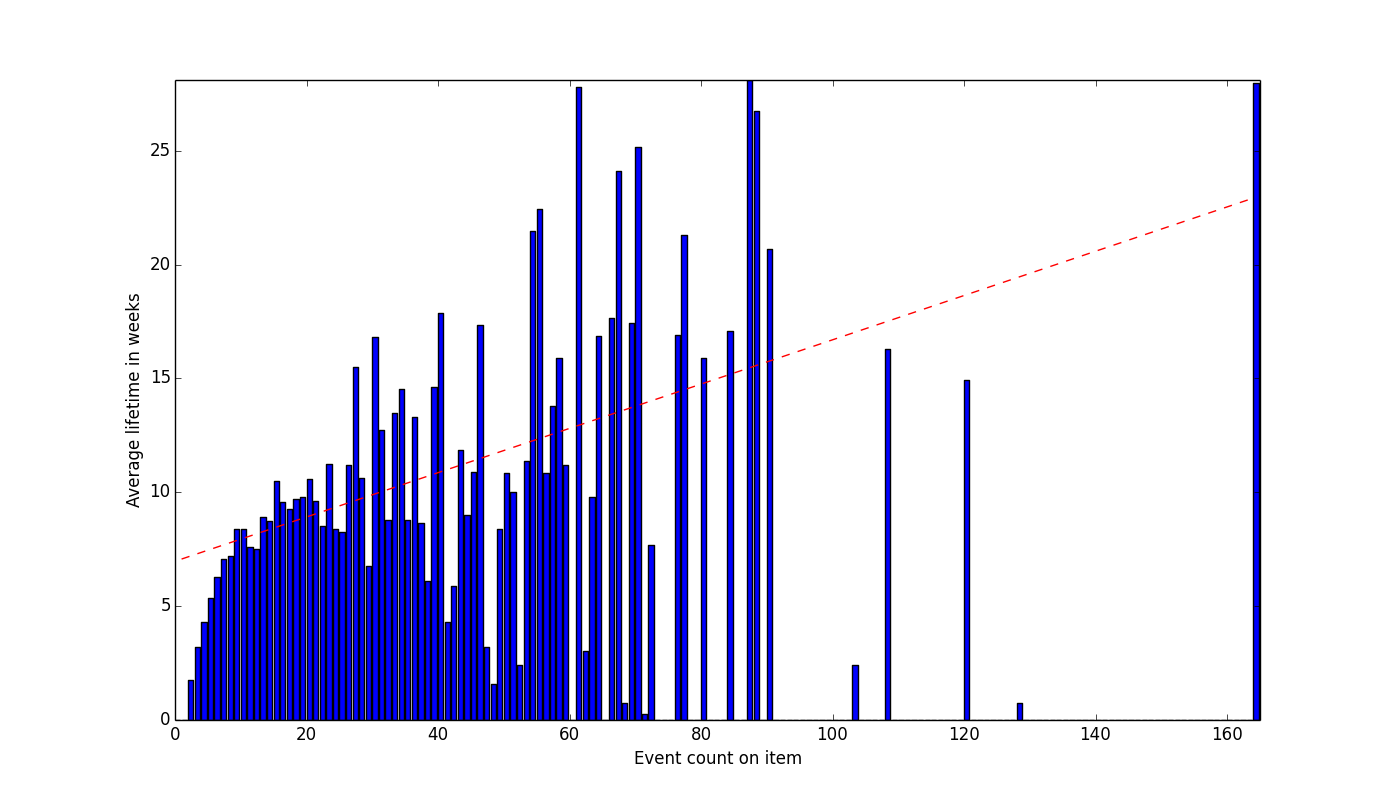
\includegraphics[width=5in]{image/avglifetimeoncount.png}
        \centering
        \caption{Average life time of items grouped on event count}
    \label{figure:averageLifetimBasedoncount}0
    \end{figure}

    \marginpar{TODO: Change x axis from minutes to days (or preferably weeks). Does this give us any hints regarding time decay factors?}
    \begin{figure}[H]
        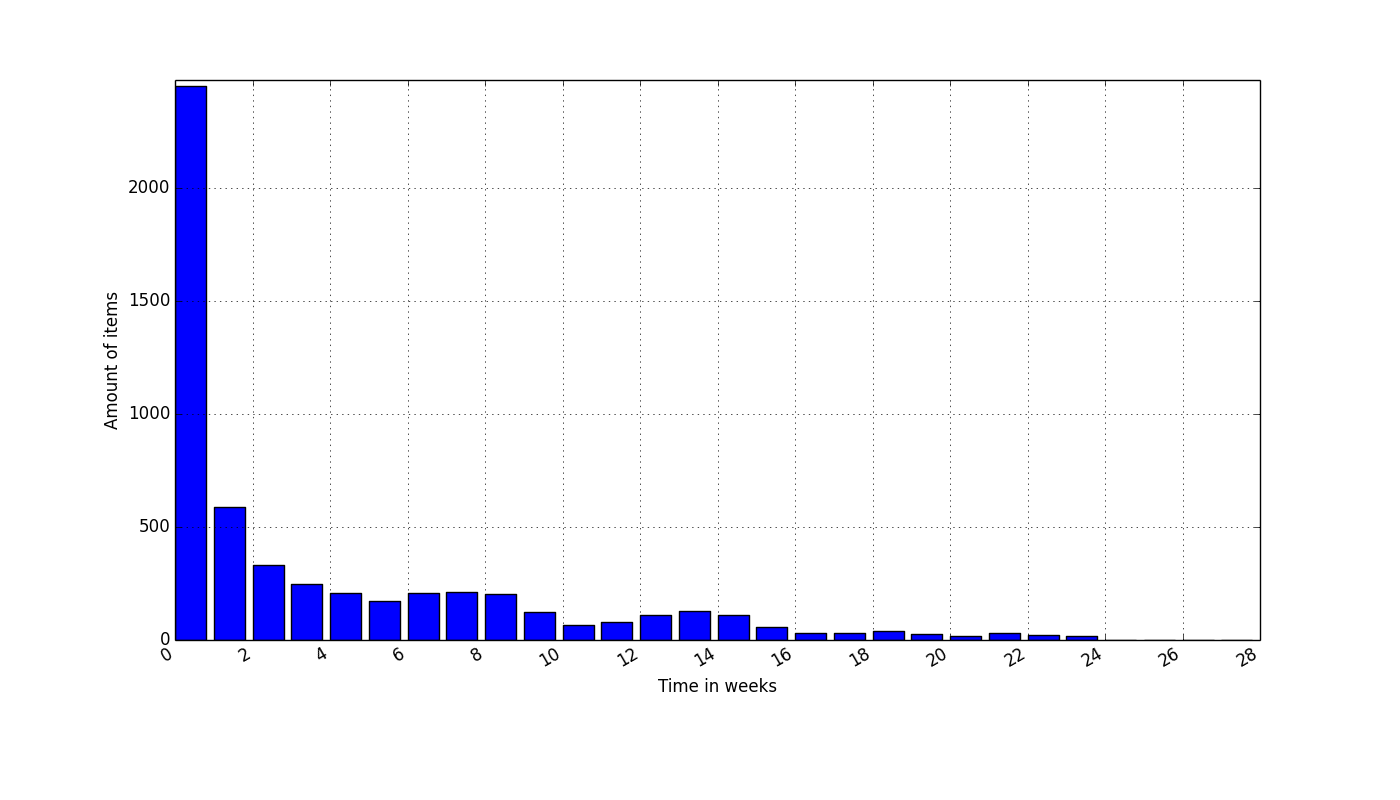
\includegraphics[width=5in]{image/itemTimespansdistribution.png}
        \centering
        \caption{Count of the different time spans of the items}
    \label{figure:itemLifes}
    \end{figure}
        This figure shows the count of items which has the different time spans.
        The numbers on the x-axis is in minutes.
        This figure makes it clearer than figure~\ref{figure:itemTimeSpanEventCount} how long the majority of the the items have lived.
        Most of the items has a time span of less than 14 000 minutes, which is less than 10 days.

    % hvorfor? er det pga:
        % a) pga veldig få events
        % b) pga kort levetid for item i datasettet
        % c) fordi det bare hadde 10 dagers "nyhetsverdi"?
    \begin{figure}[H]
        \centering
        \begin{subfigure}{.5\textwidth}
            \centering
            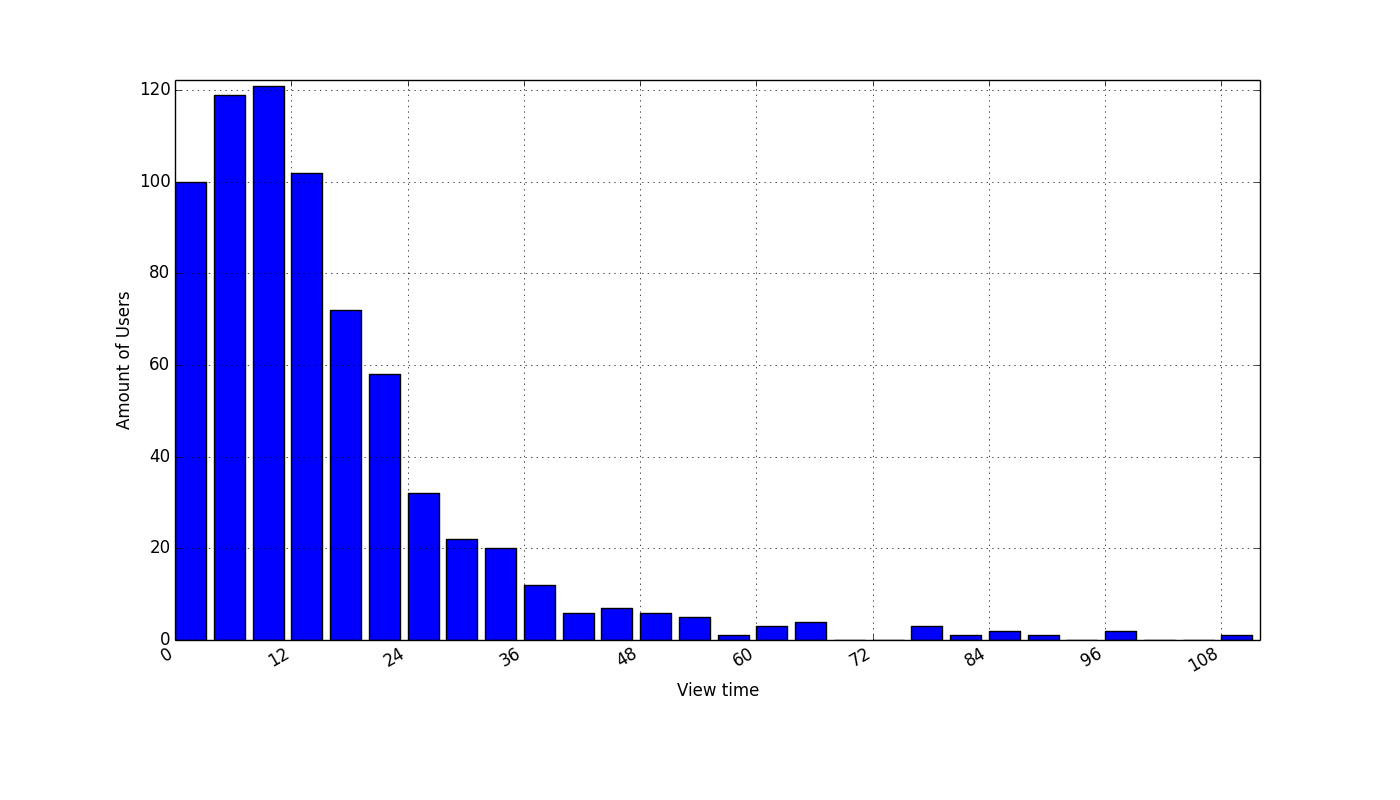
\includegraphics[width=\dualGraphWidth]{image/product_wanteddistribution.png}
            \caption{View times before wanting an item}
    \label{figure:viewWant}
        \end{subfigure}%
        \begin{subfigure}{.5\textwidth}
            \centering
            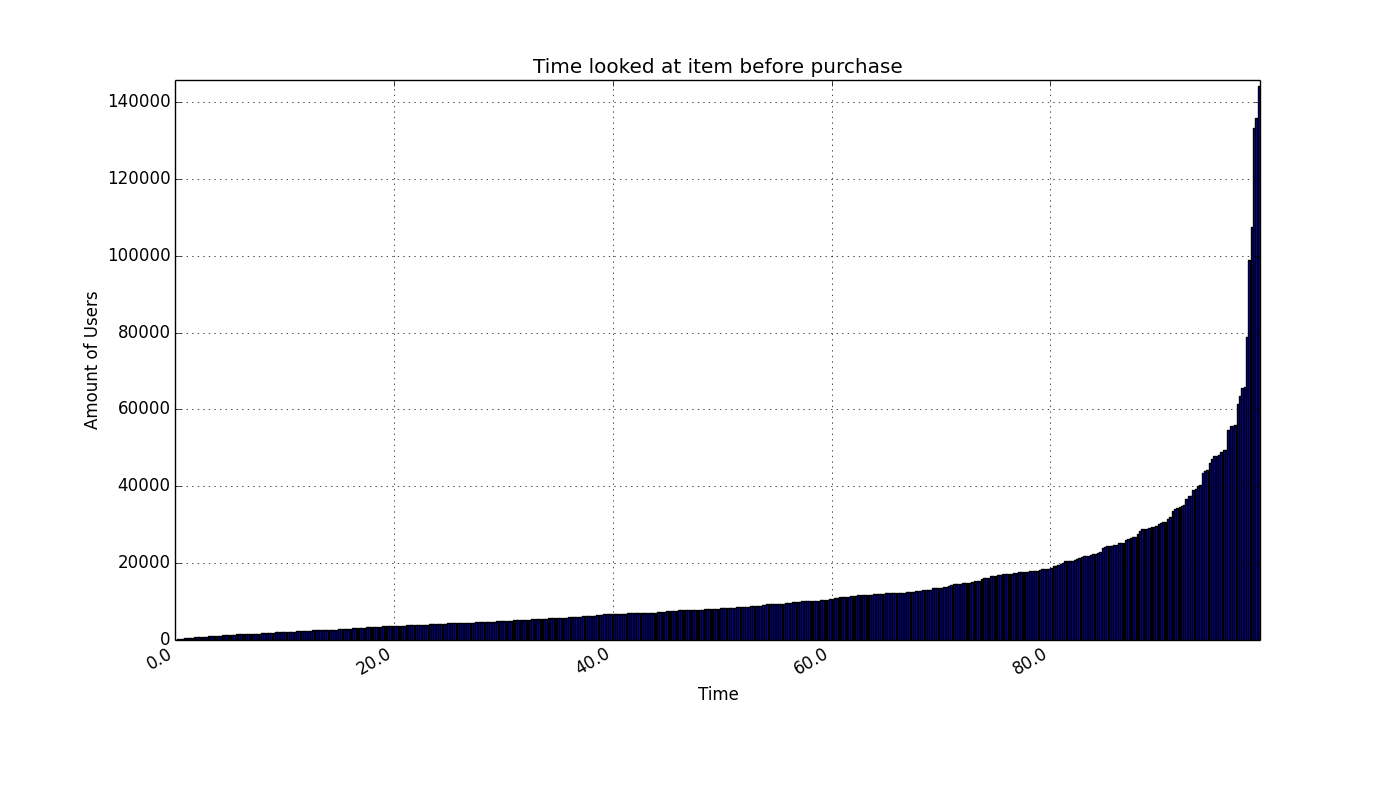
\includegraphics[width=\dualGraphWidth]{image/product_purchase_intendeddistribution.png}
            \caption{View times before purchasing an item}
    \label{figure:viewBuy}
        \end{subfigure}
        %
    \end{figure}

    % mtodo - hva betyr dette for oss? ha det i seconds, lol
    \begin{figure}[H]
        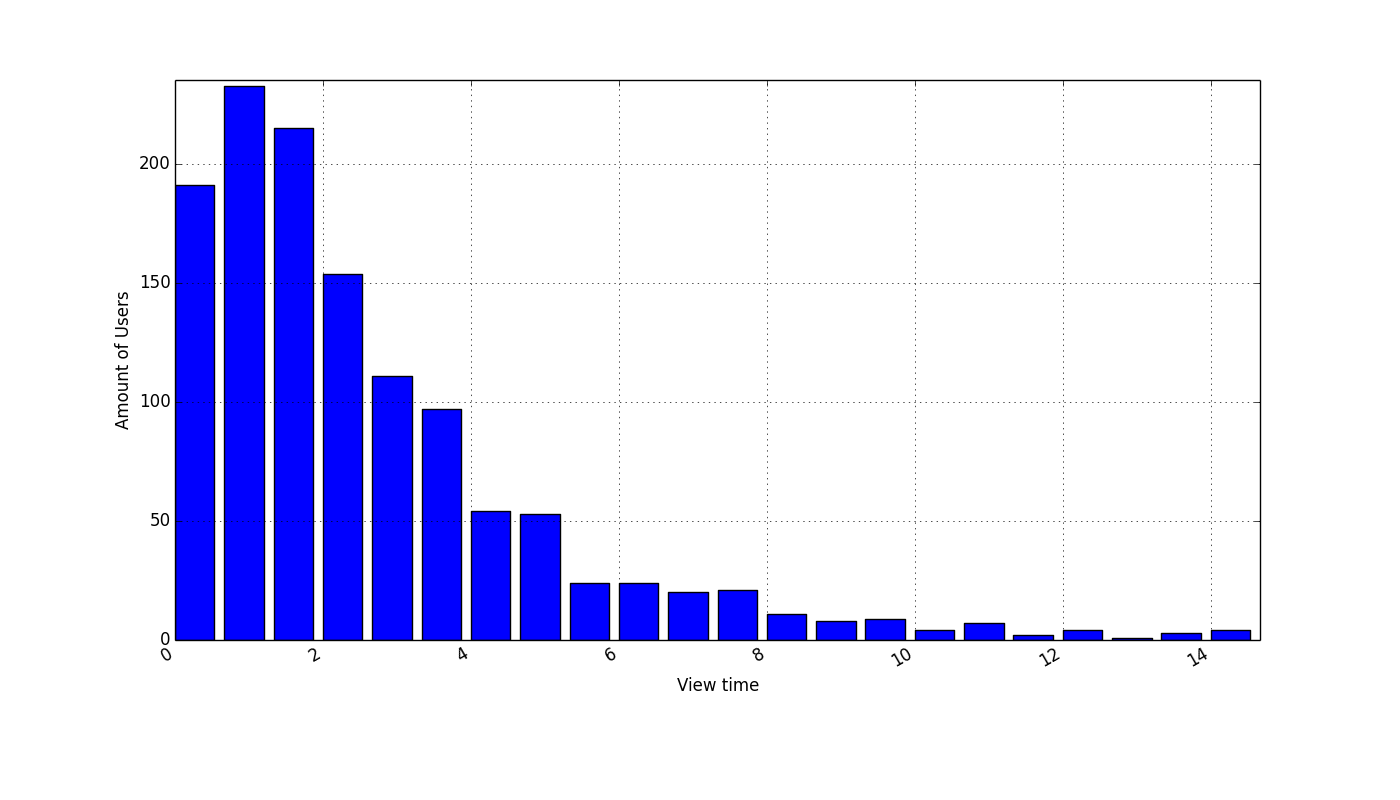
\includegraphics[width=5in]{image/product_detail_clickeddistribution.png}
        \centering
        \caption{View times before leaving an item (Bounce Rate)}
    \label{figure:bounceRate}
    \end{figure}

        This figure shows the time the users use before not taking any more action towards the item (purchase it or want it).
        The time is in milliseconds.
        The majority of the users have a view time of less than 6 000 milliseconds before they moves on to another item.

        Figure~\ref{figure:viewWant} shows the time the users use before wanting the currently viewed item.
        The time is in milliseconds.
        The majority of the users have a view time of less than 30 000 milliseconds before they want the currently viewed item.

        This figure~\ref{figure:viewBuy} shows the time the users use before purchasing the currently viewed item.
        The time is in milliseconds.
        The majority of the users have a view time of less than 32 000 milliseconds before they decide to buy the currently viewed item.

    \begin{figure}[H]
        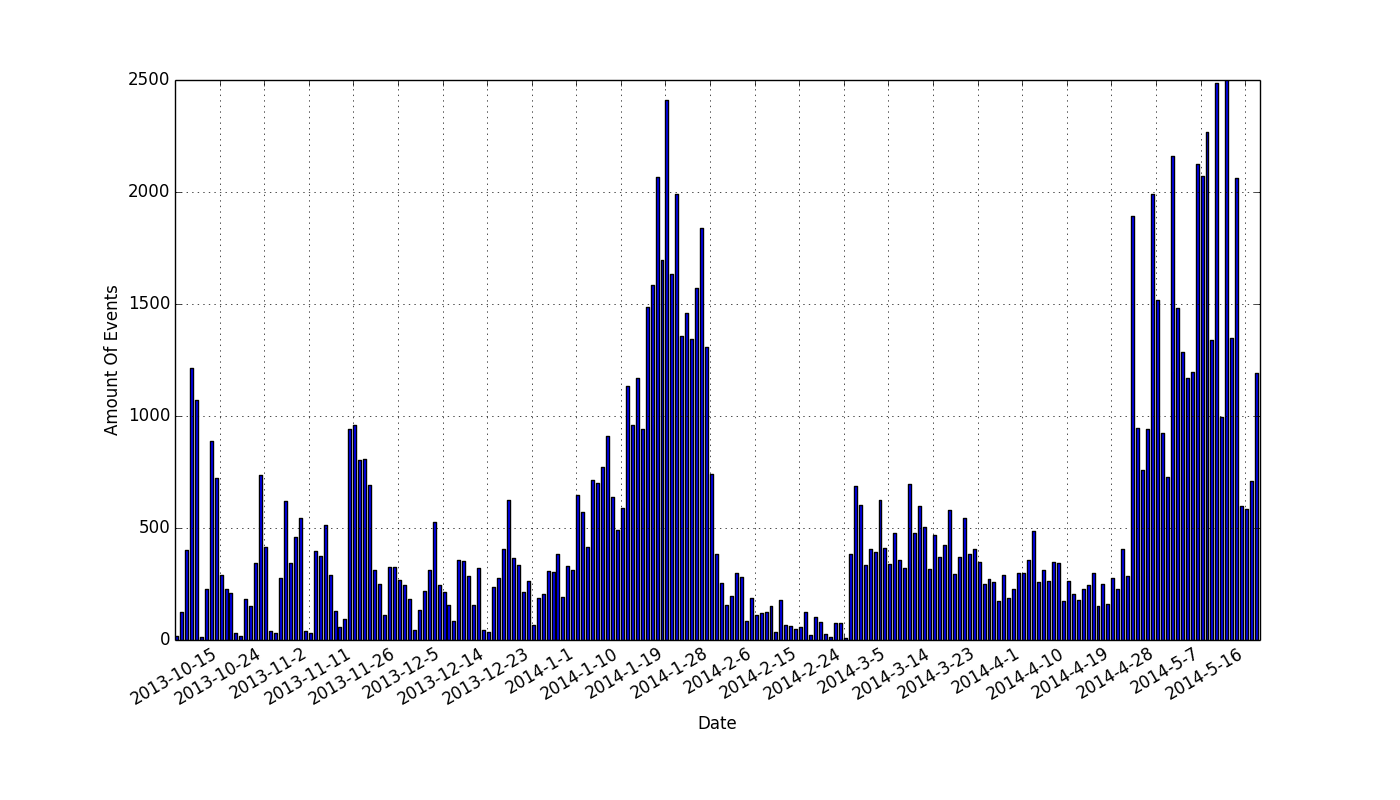
\includegraphics[width=5in]{image/eventsPerDay.png}
        \centering
        \caption{Distribution of events per day}
    \label{figure:eventOnDaysDist}
    \end{figure}
        This figure shows the event distribution per day over the time period the events were stored.
        The spikes we see happens on a weekly basis, and is centered around the weekends.
        The larger spike from the start of January to the start of March might be due to increase in publicity or other outside factors.

        % mtodo add event splits

    \begin{figure}[H]
        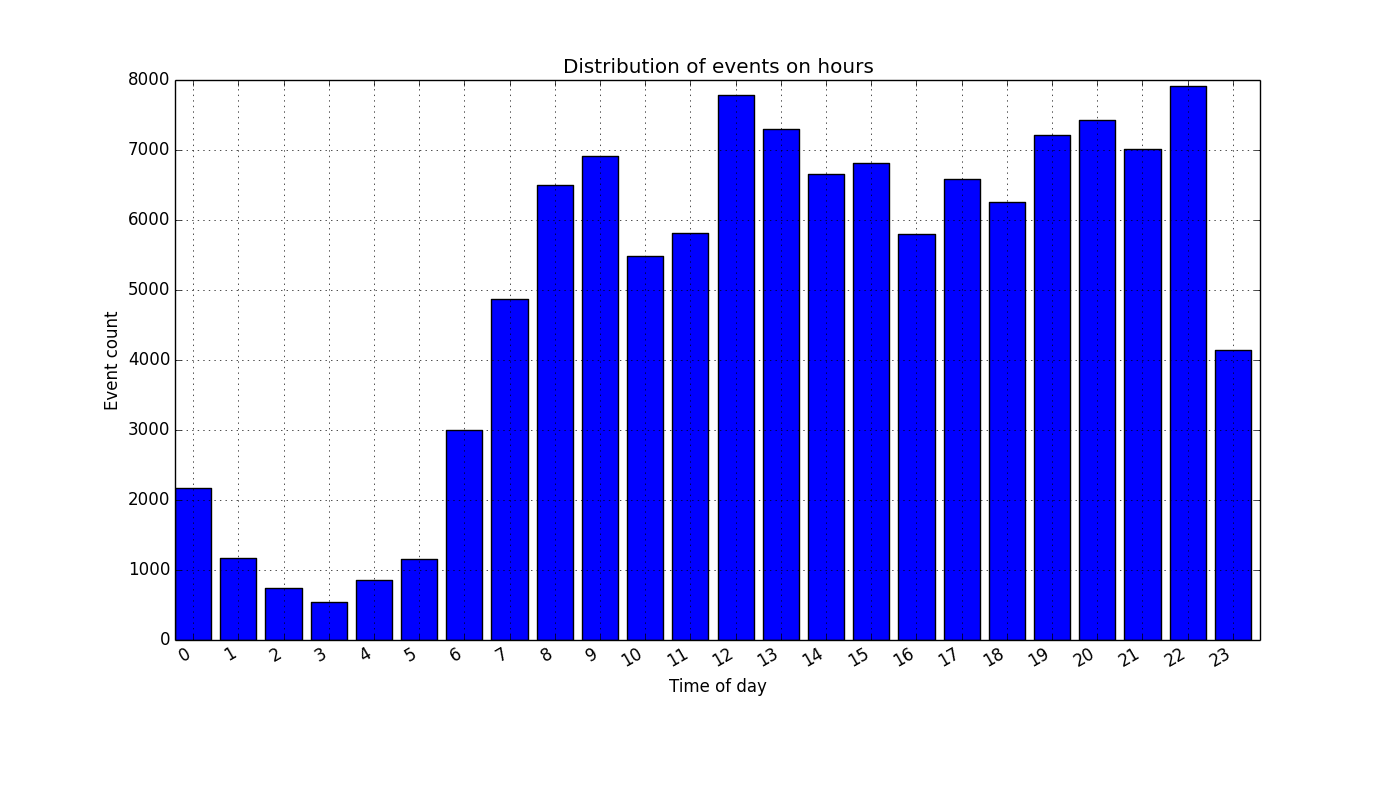
\includegraphics[width=5in]{image/hrdistribution.png}
        \centering
        \caption{mtodo}
    \label{figure:timeOfDayDistr}
    \end{figure}


\subsection{About the view time before tanking an action}
    As seen from the figures~\ref{figure:bounceRate}, ~\ref{figure:viewWant} and~\ref{figure:viewBuy}, the bounce rate is quite small compared to the time it takes for a user to decide to want or buy an item.
    This could be used as an indication of negative feedback, but since there is no explicit feedback to to test this, it might lead to rating an item negatively when the user in fact would like to rate it positively.


    %mtodo - masse fin info, men diskuter!
        % hva betyr det for oss?
        % hvordan kan data-pakket brukes av systemet?
        % dette er hands-on!
        % mange fine figurer uten konkrete beskrivelser og refereanser i teksten
        % prøv heller å lage gode forklaringer til fiugurene i teksten så referer deretter


\clearpage
\section{Conversion rate properties}

In many domains the number of activities on an item given a specific user
implies preference. The activity in question may be the number of plays in a
music service~\cite{parra2011walk} or the amount of minutes used watching a
specific TV-show~\cite{study-on-implicit-tv}. We want to validate this
hypothesis in the SoBazaar data, determining if the \textit{number of clicks}
on an item implies higher preference, that is an higher probability of buying
the item.

\marginpar{Herman: Implicit Feedback Recommendation via Implicit-to-Explicit
Ordinal Logistic Regression Mapping
 Check out related work for similar articles}


If the hypothesis holds true, we can use this fact in order improve
classification of our models in future sections. In addition we can customize
the user interface so that if a user has clicked the item, we should with a
higher frequency show the item to the user --- as he/she is more probable of
buying it once seen in detail.

In order to validate the hypothesis we iterate through all users and look at
their respective events, summarizing the number of times the user has clicked
an item $n$ times and of these how many times the user also bought it. We do
this for all values of $n$, where $n \in [1,6[$ and obtain the following table
of conversion rates and standard errors.

\begin{table}[H]
  \centering
  \begin{tabular}{lllll}
    \toprule
    N & Clicks & Purchases & Rate & Standard Error \\
    \midrule
    1 & 15602 & 1039  & 0.0667 & 0.20\% \\
    2 & 2672  & 323   & 0.1208 & 0.63\% \\
    3 & 433   & 84    & 0.1939 & 1.89\% \\
    4 & 173   & 36    & 0.2081 & 3.10\% \\
    5 & 65    & 19    & 0.2923 & 5.63\% \\
    6 & 54    & 20    & 0.3703 & 6.57\% \\
    \bottomrule
  \end{tabular}
\end{table}

The standard error gives a useful indication on how certain we can be that the
results are statisically significant, and is calculated based on the sample
size (number of clicks) and the amount of conversions. Given the rate as $r$
and sample size as $S$ we calculate the standard error $e$ as:

\begin{equation}
  e = \sqrt{\frac{r(1 - r)}{S}}
\end{equation}

Using the standard error we want to perform an hypothesis test determining if
the results are significant within our accepted confidence of 95\%. In other
words we want to be 95\% sure that the patterns found in the data are not just
random. Our two hypothesis which we want to test are thus:

$\mathbf{H_0:}$ The differences in conversion rates between our first
(baseline) and second scenerio is random.

$\mathbf{H_1:}$ The difference is significant, such that one scenario have a
higher probability of conversion.

and we want to do multiple tests when $n \in [2,6[$, using $n-1$ as baseline
and $n$ as the second scenario. For each test we calculate the
\textit{P-value}, which is the probability of obtaining a result at least as
extreme as the one that was actually observed. When the p-value becomes less
that our predetermined significance level ($0.05$ when we do a 95\%
significance test) we can reject our null-hypothesis, which is what we want to
do. In order to find this P-value we use the Standard Score, also called the
\textit{z-score}, which is the number of standard deviations an observation is
above the mean. As we have two samples we can calculate the difference in
conversion rates and use the cummulated standard error in order to find the
Z-score:

\begin{equation}
  \label{eq-z-score}
  Z = \frac{r_b - r_v}{\sqrt{e_{b}^{2} + e_{v}^{2}}}
\end{equation}

where $r_b$ and $r_v$ are the conversion rates for the baseline and second
scenario respecivly. $e_b$ and $e_v$ are equally the standard errors for the
two scenarios. Using standard normal deviate (normallly distributed random
variable with expected value 0 ($s$) and standard deviation 1 ($h$)) we can
find the cumulative probability for validity of the model - the P-value.

We calculate the P-value using $n=1$ as baseline and $n=2$ as our second
scenario. The Z-score is calculated by Equation~\ref{eq-z-score} and we obtain
our result:

\begin{equation}
  Z = \frac{0.0667-0.1208}{\sqrt{0.0020^2 + 0.0063^2}} = \frac{-0.05}{\sqrt{0.4369}} = -8.1848
\end{equation}

This is a very low Z-score, and when we are this many standard deviations away
from the mean in a standard normal deviate the P-value or area under the curve
is approximated to 0. This is a value lower than our predetermined significance
level ($0.05$) and thus we can reject the null-hypothesis and state with
statistical accuracy and correctness that there is a higher probability of
buying the item given that the user has clicked on the item twice, rather than
having clicked on the item only once. In our first scenarios we have sufficient
data to come to this conclusion, however, when comparing later scenerios we see
that our numbers stop being significant as a reult of the dataset being too
small.

\begin{table}[H]
  \centering
  \begin{tabular}{lllll}
  \toprule
  Baseline & Alternative & Z-score & P-value & Significant \\
  \midrule
  1 & 2 & -8.1848 & 0.0000 & \cmark \\
  2 & 3 & -3.6516 & 0.0001 & \cmark \\
  3 & 4 & -0.3889 & 0.3487 & \xmark \\
  4 & 5 & -1.3096 & 0.0952 & \xmark \\
  5 & 6 & -0.9013 & 0.1837 & \xmark \\
  \bottomrule
  \end{tabular}
\end{table}

Our conclusion is then that when a user has clicked on an item two times there
is a higher probability of buying it compared to when the user has only
clicked it once. This is also true when the user has clicked an item three
times, but we can not defend it statistically for any higher value of clicks.

\section{Session Findings}
    \marginpar{Something about session findings perhaps}

    % mtodo - fix caption and section :P
	\marginpar{TODO: Remove all arrows with less than e.g. 50 events}
    \begin{figure}[H]
        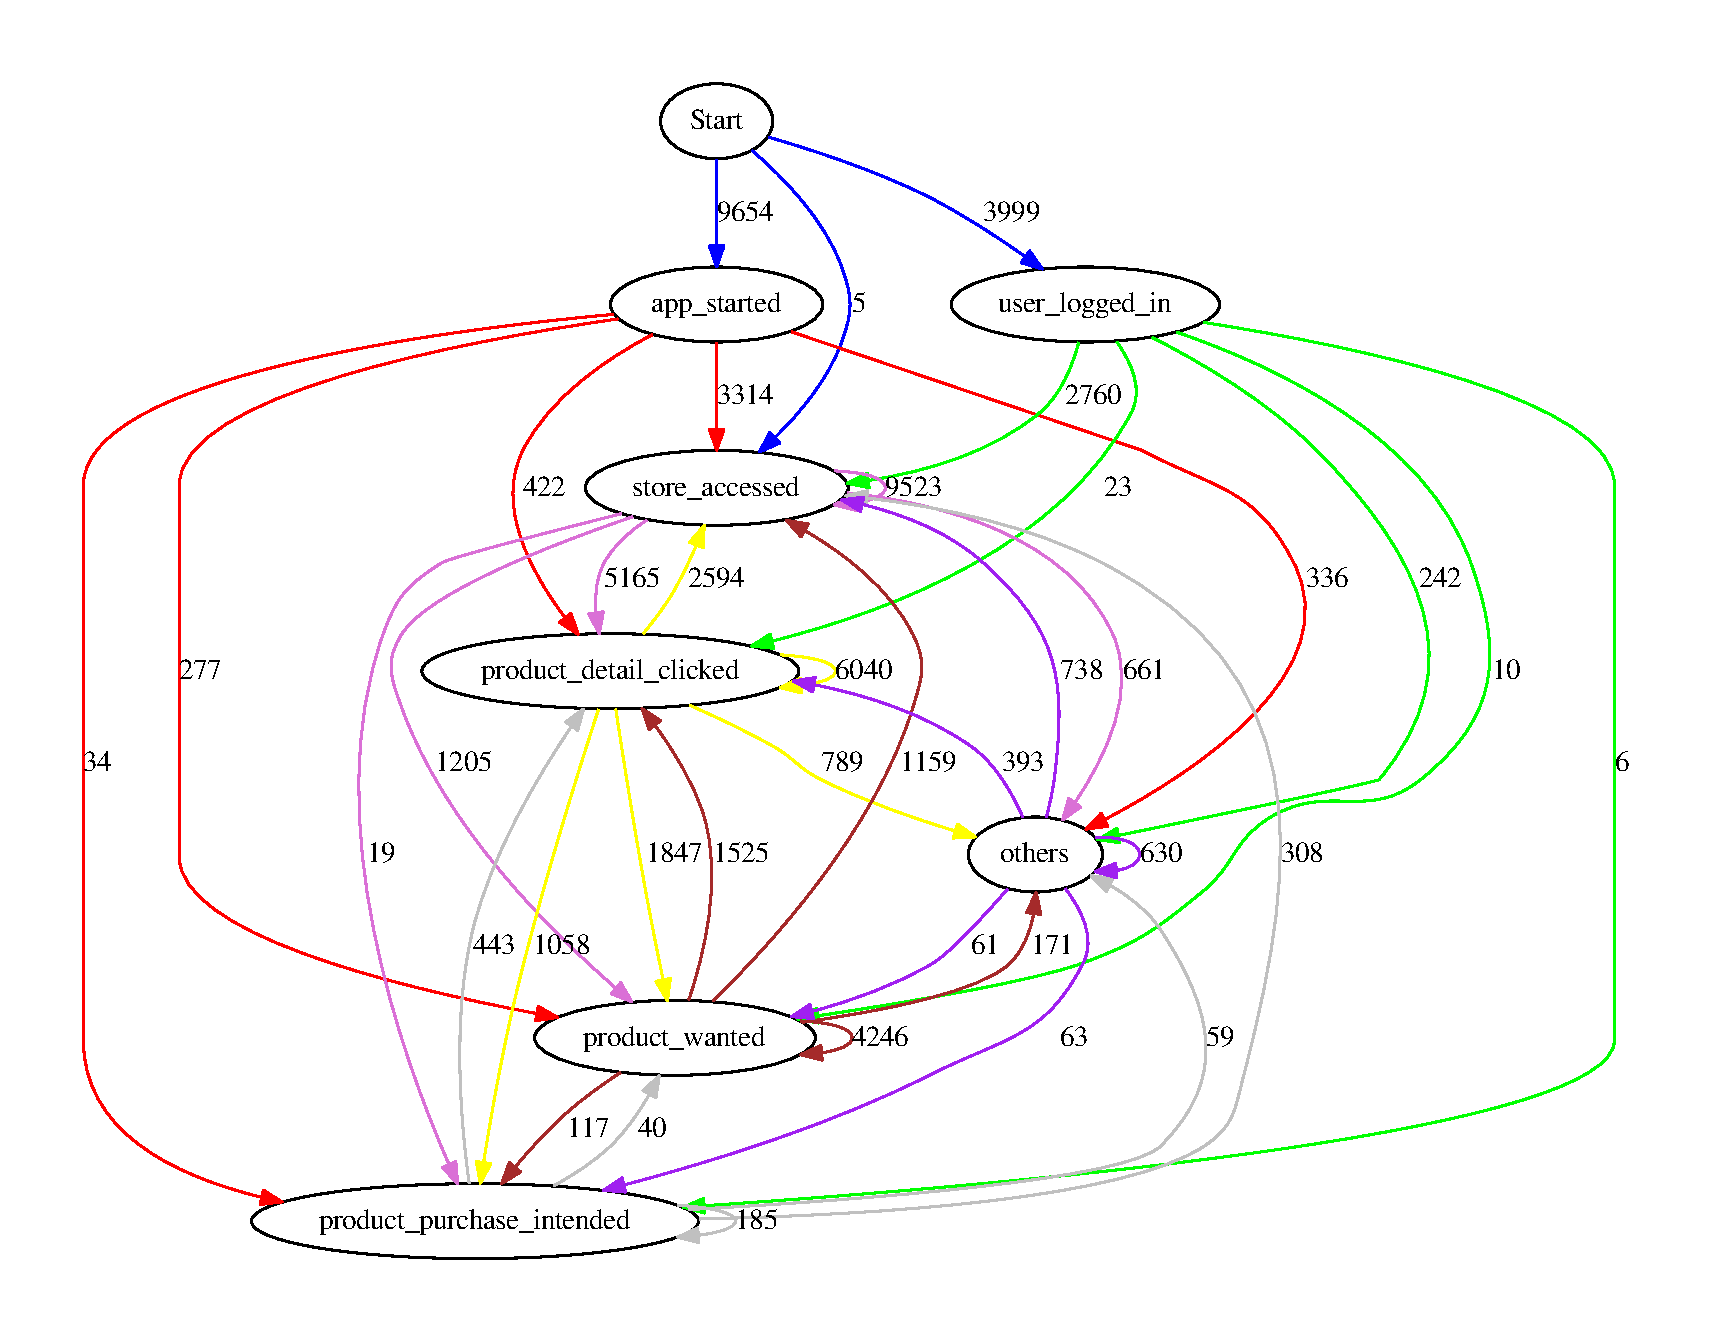
\includegraphics[width=5in]{image/statesInteractionTrue-gvfile.pdf}
        \centering
        \caption{A minimized view of the different states of the system and how they interact with each other.}
        \label{figure:minStatesInteractions}
    \end{figure}

    Full view see~\ref{figure:statesInteractions}

    \begin{figure}[H]
        \centering
        \begin{subfigure}{.33\textwidth}
            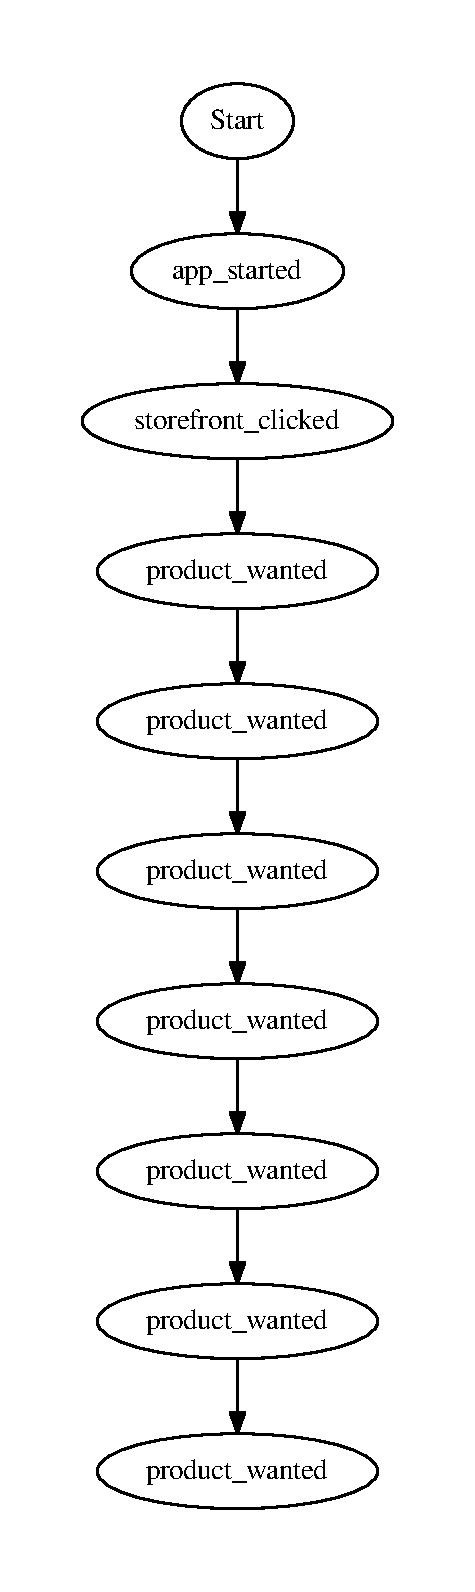
\includegraphics[width=2in]{image/403session-2-gvfile.pdf}
            \centering
            \caption{mtodo}
    \label{subfigure:statesInteractions}
        \end{subfigure}%
        \begin{subfigure}{.33\textwidth}
            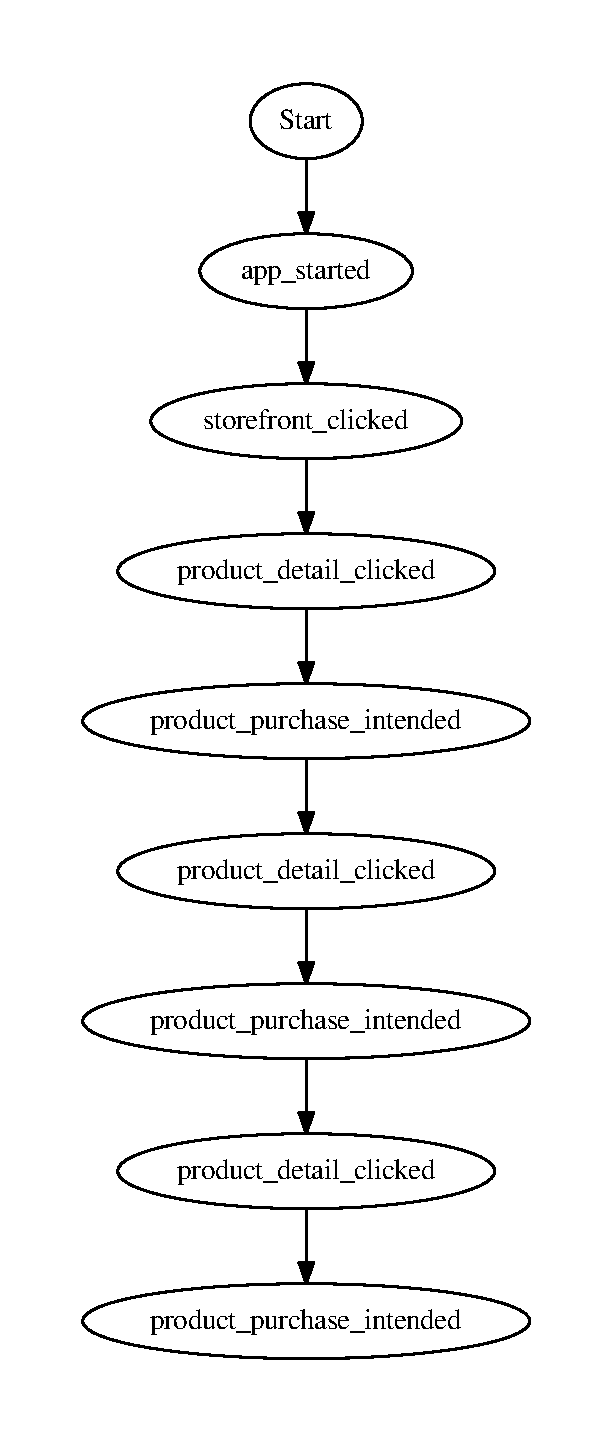
\includegraphics[width=2in]{image/309session-3-gvfile.pdf}
            \centering
            \caption{mtodo}
    \label{subfigure:statesInteractions}
        \end{subfigure}%
        \begin{subfigure}{.33\textwidth}
            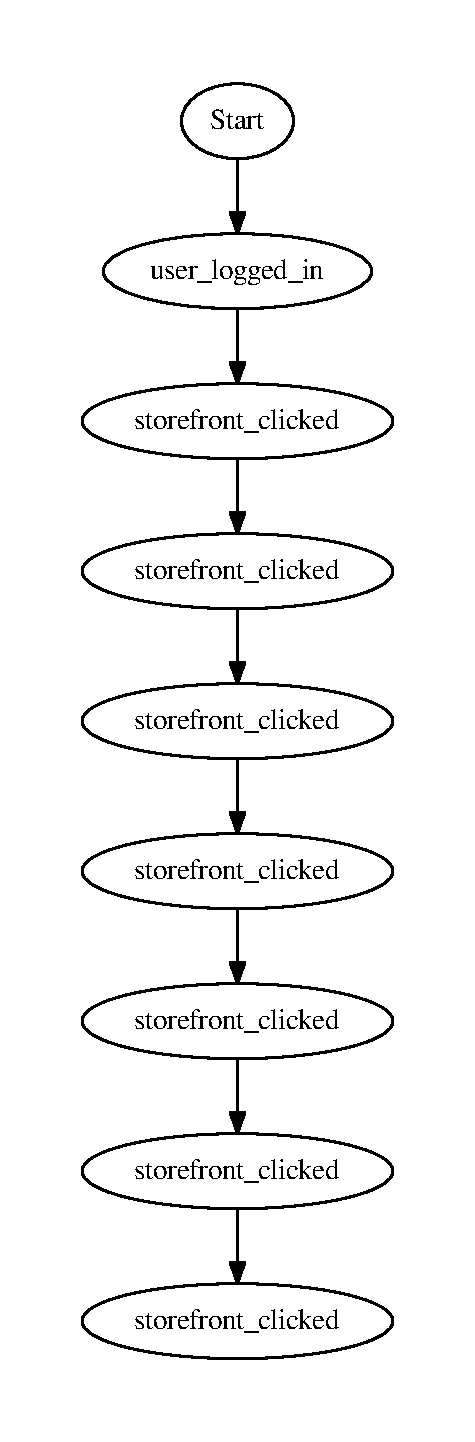
\includegraphics[width=2in]{image/56session-17-gvfile.pdf}
            \centering
            \caption{mtodo}
    \label{subfigure:statesInteractions}
        \end{subfigure}
        %
    \end{figure}

    % mtodo - fix lol
%     Init Hypothesis:
%     Two users with similar session habits and similar product accessing pattern
%     have a stronger correlation to one-another than two users with just similar
%     product interests.


%     'product\_purchase\_intended' (user pushed to the product web store) shows a
%     wider specter of information about the product, including additional colors,
%     images and colors.  For some it might be natural to explore the item there
%     before "wanting" it. Making both

%     "product\_purchase\_intended" $\Rightarrow$ "product\_wanted"

%     and

%     "product\_purchase\_intended" $\notimplies$ "product\_wanted"

%     produce valuable information.

%     Must make different rules for the different stores:
%     "Bik Bok", "Cubus", "Gina Trik", "H\&M", "Bianco" has a broad specter of extra
%     functions inside the web store, whereas others might not, only shows the
%     product and a add to chart button.  This might divide the use pattern of the
%     users into a:

%     "product\_detail\_clicked" $\Rightarrow$ "product\_purchase\_intended" $\Rightarrow$ "product\_wanted"

%     "product\_detail\_clicked" $\Rightarrow$ "product\_purchase\_intended" $\notimplies$ "product\_wanted",

%     and

%     "product\_detail\_clicked" $\Rightarrow$ "product\_wanted"

%     based on the store accessed.

%     Use this to make a "rule set" with a probability.
%     Then again use this to recommend items for the users with that given
%     probability.

%     Find a "most popular session"-pattern
%     Find a "most likely to come after"-pattern

%     Session issues:
%     Once in a blue moon a user will do a "product action" (purchase,want,details)
%     without having a previous frontstore-access event. Which leads to unknown
%     store-id of the item.

%     Issue is most probably from missing user-id in collection\_viewed, and a user
%     checks out an item from there. It is not possible to be 100\% sure which user
%     access the item from the collection\_viewed event, so this event is therefor
%     not integrated into the session-stack.


\section{Conclusion}
\ref{sec:dataset-conclusion}

%Summarize the findings
%What can be used?

